% !TeX TXS-program:bibliography = txs:///biber
% chktex-file 1
\documentclass[fontsize=14pt, russian]{scrartcl}
\input{header.tex}
\addbibresource{biblio.bib}

\usepackage{svg}

\newlength{\lblwd}
\newcommand{\titlefield}[2]{%
  \par\addvspace{1.6ex}%
  \settowidth{\lblwd}{\small #1}%
  \noindent\small #1\hspace{1em}%
  \underline{\makebox[\dimexpr\linewidth-\lblwd-1em\relax][l]{\small #2}}%
  \par
}

\begin{document}
\sloppy

\def\figurename{Рисунок}

\newcommand{\sqlkw}[1]{\texttt{#1}}
\newcommand{\SELECT}{\sqlkw{SELECT}}
\newcommand{\FROM}{\sqlkw{FROM}}
\newcommand{\WHERE}{\sqlkw{WHERE}}
\newcommand{\JOIN}{\sqlkw{JOIN}}
\newcommand{\GROUPBY}{\sqlkw{GROUP BY}}
\newcommand{\ORDERBY}{\sqlkw{ORDER BY}}

\newcommand{\COUNT}{\sqlkw{COUNT}}
\newcommand{\SUM}{\sqlkw{SUM}}
\newcommand{\AVG}{\sqlkw{AVG}}
\newcommand{\MIN}{\sqlkw{MIN}}
\newcommand{\MAX}{\sqlkw{MAX}}

\newcommand{\LogicalGet}{\sqlkw{LogicalGet}}
\newcommand{\SeqScan}{\sqlkw{SeqScan}}
\newcommand{\IndexScan}{\sqlkw{IndexScan}}
\newcommand{\NestedLoopJoin}{\sqlkw{NestedLoopJoin}}
\newcommand{\NestedLoopCrossJoin}{\sqlkw{NestedLoopCrossJoin}}
\newcommand{\HashJoin}{\sqlkw{HashJoin}}
\newcommand{\MergeJoin}{\sqlkw{MergeJoin}}
\newcommand{\Sort}{\sqlkw{Sort}}
\newcommand{\FilterOp}{\sqlkw{Filter}}
\newcommand{\ProjOp}{\sqlkw{Projection}}

\newcommand{\SelOp}[1]{\sigma_{#1}}
\newcommand{\ProjectionOp}[1]{\pi_{#1}}

\newcommand{\Sel}[2]{\sigma_{#1}(#2)}
\newcommand{\Projection}[2]{\pi_{#1}(#2)}
\newcommand{\Agg}[3]{\gamma_{#1;\,#2}(#3)}
\newcommand{\AggP}[3]{\gamma_{#1;\,#2}^{partial}(#3)}
\newcommand{\NJoin}[2]{#1 \bowtie #2}
\newcommand{\InnerJoin}[3]{#1 \bowtie_{#2} #3}
\newcommand{\CProd}[2]{#1 \times #2}
\newcommand{\LOJ}[3]{#1 \ltimes_{#2} #3}
\newcommand{\ROJ}[3]{#1 \rtimes_{#2} #3}
\newcommand{\FOJ}[3]{#1 \mathbin{\ltimes\!\!\!\rtimes}_{#2} #3}
\newcommand{\Tr}[1]{[\![ #1 ]\!]}
\newcommand{\Apply}[2]{#1 \mathbin{\mathcal{A}} #2}
\newcommand{\TransRule}[3]{%
  \ensuremath{%
    \begin{array}{c}
      #1 \\[1pt]
      \xRightarrow{\,#2\,} \\[1pt]
      #3
    \end{array}%
  }%
}

\begin{titlepage}
	\thispagestyle{empty}
	\newpage

	\vspace*{-30pt}
	\hspace{-45pt}
	\begin{minipage}{0.17\textwidth}
		\hspace*{-20pt}\centering
		\includegraphics[width=1.3\textwidth]{emblem.png}
	\end{minipage}
	\begin{minipage}{0.82\textwidth}\small \textbf{
			\vspace*{-0.7ex}
			\hspace*{-10pt}\centerline{Министерство науки и высшего образования Российской Федерации}
			\vspace*{-0.7ex}
			\centerline{Федеральное государственное автономное образовательное учреждение }
			\vspace*{-0.7ex}
			\centerline{высшего образования}
			\vspace*{-0.7ex}
			\centerline{<<Московский государственный технический университет}
			\vspace*{-0.7ex}
			\centerline{имени Н.Э. Баумана}
			\vspace*{-0.7ex}
			\centerline{(национальный исследовательский университет)>>}
			\vspace*{-0.7ex}
			\centerline{(МГТУ им. Н.Э. Баумана)}}
	\end{minipage}

	\vspace{-2pt}
	\hspace{-34.5pt}\rule{\textwidth}{2.5pt}

	\vspace*{-20.3pt}
	\hspace{-34.5pt}\rule{\textwidth}{0.4pt}

\titlefield{ФАКУЛЬТЕТ}{<<Информатика и системы управления>>}
\titlefield{КАФЕДРА}{<<Теоретическая информатика и компьютерные технологии>>}


\vspace{3em}
\begin{center}
    {\Large\bfseries РАСЧЕТНО-ПОЯСНИТЕЛЬНАЯ ЗАПИСКА}\\[1.5ex]
    {\Large\bfseries\itshape К ВЫПУСКНОЙ КВАЛИФИКАЦИОННОЙ РАБОТЕ НА ТЕМУ:}\\[1.5ex]
    {\large\bfseries\itshape <<Автоматическая оптимизация планов выполнения SQL-запросов>>}
\end{center}

\vspace{\fill}


	\newlength{\ML}
	\settowidth{\ML}{«\underline{\hspace{0.7cm}}» \underline{\hspace{2cm}}}

	\noindent Студент \underline{\text{ИУ9-81Б}} \hfill \underline{ \hspace{4cm}}\quad
	\raisebox{0.42ex}{\underline{\parbox{4cm}{\centering Старовойтов А. И.}}}

	\vspace{-0.5ex}
	\noindent\hspace{9ex}\scriptsize{(Группа)}\normalsize\hspace{170pt}\hspace{2ex}\scriptsize{(Подпись, дата)}\normalsize\hspace{30pt}\hspace{6ex}\scriptsize{(Фамилия И.О.)}\normalsize

	\bigskip

	\noindent Научный руководитель  \hfill \underline{\hspace{4cm}}\quad
	\raisebox{0.3ex}{\underline{\parbox{4cm}{\centering Непейвода А. Н.}}}

	\vspace{-0.5ex}
	\noindent\hspace{13.5ex}\normalsize\hspace{170pt}\hspace{2ex}\scriptsize{(Подпись, дата)}\normalsize\hspace{30pt}\hspace{6ex}\scriptsize{(Фамилия И.О.)}\normalsize

	\bigskip

	\noindent Нормоконтролёр  \hfill \underline{\hspace{4cm}}\quad
	\raisebox{0.15ex}{\underline{\parbox{4cm}{\centering Алексеев С. М.}}}

	\vspace{-0.5ex}
	\noindent\hspace{13.5ex}\normalsize\hspace{170pt}\hspace{2ex}\scriptsize{(Подпись, дата)}\normalsize\hspace{30pt}\hspace{6ex}\scriptsize{(Фамилия И.О.)}\normalsize

	\vfill

	%\vspace{\fill}



	\begin{center}
		\textsl{2026}
	\end{center}
\end{titlepage}

\setlength{\tabcolsep}{3pt}
\setcounter{page}{2}
%----------------------------------------------------------------------------
%                  ОТСЮДА --- СОБСТВЕННО ТЕКСТ
%----------------------------------------------------------------------------
\section*{АННОТАЦИЯ}

Работа посвящена разработке оптимизатора SQL-запросов для модельной реляционной
СУБД. Цель работы состоит в реализации оптимизатора на основе архитектуры
Cascades и создании основы для его дальнейшего улучшения за счет сопоставления
порождаемых физических планов с планами промышленных систем.

В ходе исследования рассмотрены архитектуры оптимизаторов System~R, Volcano и
Cascades, формализовано поддерживаемое подмножество SQL и соответствующее ему
подмножество реляционной алгебры. При реализации использованы структура Memo,
правила логических преобразований и физических реализаций, стоимостная модель,
учет требуемых физических свойств, а также метод ветвей и границ для отсечения
неперспективных вариантов планов. Для оценки работы системы применены модульное
тестирование, генерация SQL-запросов, бенчмарки физических операторов и
дифференциальное сравнение планов с Microsoft SQL Server.

В результате разработана модельная СУБД, работающая с CSV-файлами и
поддерживающая основные операторы реляционной алгебры, а также расширяемый
оптимизатор, способный строить физические планы с учетом стоимости и физических
свойств результата. Получены стоимостные формулы операторов, подтвержден прирост
производительности относительно наивного плана и подготовлены инструменты для
поиска случаев, в которых пространство поиска оптимизатора требует расширения.
Практическая значимость работы заключается в возможности использовать
реализованную систему как основу для экспериментального исследования методов
оптимизации запросов и итеративного развития набора правил оптимизатора.

\newpage
\renewcommand\contentsname{\hfill{\normalfont{СОДЕРЖАНИЕ}}\hfill}
\tableofcontents
\newpage
\anonsection{ВВЕДЕНИЕ}

В эпоху стремительного роста объемов данных системы управления базами данных
(СУБД) являются важной частью информационных систем. По данным аналитических
исследований, объем мирового рынка СУБД ежегодно увеличивается, что обусловлено
как расширением круга решаемых задач, так и усложнением структуры обрабатываемых
данных и увеличением их объема. Реляционные базы данных, работающие с различными
диалектами языка SQL, продолжают занимать доминирующее положение в сегменте
обработки транзакций и аналитических запросов.

Одним из определяющих факторов конкурентоспособности между различными
реализациями СУБД является качество оптимизатора запросов. Оптимизатор
представляет собой компонент, ответственный за преобразование декларативного
SQL-запроса в эффективный физический план исполнения. Именно от качества работы
оптимизатора в значительной степени зависит производительность всей системы:
выбор неоптимального плана исполнения может привести к увеличению времени
выполнения запроса в десятки раз относительно оптимального случая.Также
оптимизатор запросов считается наиболее сложной составной частью любой СУБД.
Задача нахождения оптимального плана является NP-полной в общем случае, что
обуславливает необходимость применения эвристических методов и алгоритмов
ограниченного перебора.

Архитектура оптимизаторов Cascades используется в таких промышленных системах,
как Microsoft SQL Server, Apache Orca, а также в ряде исследовательских
проектов, включая Columbia и CockroachDB\@. Преимущества этой архитектуры
заключаются в расширяемости, модульности, а также понятном и эффективном
алгоритме поиска, допускающим параллельность исполнения.

Целью данной работы является разработка и реализация оптимизатора подмножества
SQL-запросов на основе архитектуры Cascades, а также создание каркаса для его
итеративного улучшения путем сравнения с промышленными реализациями.

Для достижения поставленной цели прежде всего требуется изучить архитектуру
оптимиазторов Cascades и на ее основе проработать собственную.

После выбора архитектурной основы необходимо формализовать поддерживаемое
подмножество SQL и соответствующее ему подмножество реляционной алгебры. Эта
задача определяет границы рассматриваемых запросов, их семантику и внутреннее
логическое представление, используемое на этапе оптимизации.

Следующим шагом является реализация структуры данных Memo и алгоритма поиска
оптимального физического плана на основе архитектуры Cascades. В рамках этой
задачи требуется обеспечить хранение эквивалентных логических выражений,
повторное использование найденных вариантов планов и выбор плана с минимальной
оценочной стоимостью.

Чтобы сформировать пространство поиска оптимизатора, требуется разработать набор
правил трансформации и реализации для основных операторов реляционной алгебры.
Правила трансформации должны порождать логически эквивалентные планы, а правила
реализации сопоставлять логическим операторам допустимые физические операторы.

Для оптимизации алгоритма поиска нужно реазивовать метод ветвей и границ. Этот
метод должен использовать оценки стоимости для отсечения заведомо неоптимальных
планов и уменьшения объема пространства поиска, исследуемого оптимизатором.

Для последующего развития системы также требуется реализовать метод
дифференциального анализа физических планов. Он должен обеспечивать
автоматизированный поиск примеров неоптимальных планов путем сравнения планов
разрабатываемого оптимизатора с планами промышленных СУБД, а найденные различия
должны использоваться для уточнения правил оптимизации.

\section{Исследовательская часть}

Система управления базами данных представляет собой программный комплекс,
обеспечивающий хранение, извлечение и модификацию структурированных
данных. Несмотря на разнообразие существующих реализаций, архитектура
большинства реляционных СУБД включает ряд типовых компонентов,
взаимодействие которых обеспечивает выполнение пользовательских запросов.

К основным компонентам СУБД относятся~\refImage{fig::dbms_arch}:

\begin{itemize}
    \item транспортный уровень, принимающий клиентские подключения и запросы;
    \item синтаксический анализатор (парсер), выполняющий разбор текста
SQL-запроса и построение синтаксического дерева;
    \item оптимизатор запросов, преобразующий логическое представление запроса в
эффективный физический план исполнения;
    \item исполнитель, непосредственно реализующий физический план;
    \item менеджер хранения данных, управляющий размещением данных на физических
носителях;
    \item менеджер транзакций и менеджер блокировок, обеспечивающие гарантии
транзакций;
    \item менеджер страниц памяти, отвечающий за кэширование страниц данных в
оперативной памяти.
\end{itemize}

\begin{figure}[!htb]\centering
\usetikzlibrary{fit}
\begin{tikzpicture}[
    box/.style={rectangle, draw, minimum width=4.1cm, minimum height=1cm,
                align=center, font=\small},
    wbox/.style={rectangle, draw, minimum width=9.1cm, minimum height=1cm,
                 align=center, font=\small},
    grp/.style={draw, dashed, inner sep=0.3cm},
    lbl/.style={font=\small},
]
    \node[box] (clust)   at (-2.5,  0)    {Кластерные\\соединения};
    \node[box] (client)  at ( 2.5,  0)    {Клиентские\\соединения};
    \node[grp, fit=(clust)(client)] (TG) {};
    \node[lbl, anchor=south west] at (TG.north west) {Транспорт};

    \node[wbox]               (parser) at (0, -2.8)  {Синтаксический анализатор};
    \node[wbox, fill=gray!20] (optim)  at (0, -4.05) {\textbf{Оптимизатор запросов}};
    \node[grp, fit=(parser)(optim)] (QPG) {};
    \node[lbl, anchor=south west] at (QPG.north west) {Обработчик запросов};

    \node[box] (remote)  at (-2.5, -6.85) {Удалённое\\исполнение};
    \node[box] (local)   at ( 2.5, -6.85) {Локальное\\исполнение};
    \node[grp, fit=(remote)(local)] (EEG) {};
    \node[lbl, anchor=south west] at (EEG.north west) {Исполнитель};

    \node[box]  (txmgr)   at (-2.5,  -9.65) {Менеджер\\транзакций};
    \node[box]  (lockmgr) at ( 2.5,  -9.65) {Менеджер\\блокировок};
    \node[wbox] (access)  at (   0, -10.9)  {Методы доступа};
    \node[box]  (bufmgr)  at (-2.5, -12.15) {Менеджер\\страниц};
    \node[box]  (recmgr)  at ( 2.5, -12.15) {Менеджер\\восстановления};
    \node[grp, fit=(txmgr)(lockmgr)(access)(bufmgr)(recmgr)] (SEG) {};
    \node[lbl, anchor=south west] at (SEG.north west) {Подсистема хранения};

    \draw[<->, thick, >=stealth]
        ([xshift=0.4cm]TG.south  east) -- ([xshift=0.4cm]QPG.north east);
    \draw[<->, thick, >=stealth]
        ([xshift=0.4cm]QPG.south east) -- ([xshift=0.4cm]EEG.north east);
    \draw[<->, thick, >=stealth]
        ([xshift=0.4cm]EEG.south east) -- ([xshift=0.4cm]SEG.north east);

    \draw[thick] ([xshift=-0.5cm]clust.west)  -- ([xshift=-0.5cm]remote.west);
    \draw[->, thick, >=stealth] ([xshift=-0.5cm]clust.west)  -- (clust.west);
    \draw[->, thick, >=stealth] ([xshift=-0.5cm]remote.west) -- (remote.west);
\end{tikzpicture}
    \caption{Архитектура реляционной системы управления базами данных}%
    \label{fig::dbms_arch}
\end{figure}

\subsection{Процесс исполнения SQL-запроса}

Процесс исполнения SQL-запроса в реляционной СУБД проходит несколько
последовательных этапов.

\begin{enumerate}
  \item \emph{Синтаксический анализ} --- запроса проходит лексический и
        синтаксический разбор. Результатом данного этапа является синтаксическое
        дерево, узлы которого соответствуют конструкциям языка SQL: операторам
        \SELECT, \FROM, \WHERE, \JOIN, \GROUPBY, \ORDERBY{} и другим. На этом же
        этапе выполняется семантический анализ: проверяется существование
        указанных таблиц и столбцов, разрешаются имена объектов и определяются
        типы выражений.

  \item \emph{Оптимизация} --- синтаксическое дерево преобразуется в логический
        план запроса, выраженный в терминах реляционной алгебры. Оптимизатор
        исследует пространство эквивалентных логических планов и для каждого из
        них рассматривает возможные физические реализации операторов. С помощью
        модели стоимости оптимизатор оценивает затраты на выполнение каждого
        плана и выбирает план с наименьшей оценочной стоимостью. Результатом
        этого этапа является физический план исполнения. Под этим понимается
        дерево физических операторов с указанием конкретных алгоритмов
        соединения, методов доступа к данным и порядка операций.

  \item \emph{Исполнение физического плана} --- движок выполнения реализует
        физический план, порождая потоки кортежей. Данные извлекаются из
        хранилища, обрабатываются операторами плана и формируют результирующий
        набор, возвращаемый пользователю.
\end{enumerate}


Сформулируем задачу, которую решает оптимизатор: по запросу, представленному в
форме дерева операторов реляционной алгебры, построить эквивалентный и
оптимальный, с точки зрения необходимых для исполнения ресурсов, план
исполнения. Итоговый план является деревом, вершины которого помечены
конкретными указаниями на алгоритмы, реализующими один или несколько операторов
реляционной алгебры. Эквивалентность означает, что итоговый физический план и
исходный запрос при исполнении на любом наборе данных порождают одинаковые
отношения с точностью до требуемых свойств, таких как сортировка.

Запрос в форме реляционной алгебры также называют логическим планом, а операторы
реляционной алгебры --- логическими операторами.

Для каждого логического оператора существует несколько возможных физических
реализаций. Например, оператор соединения \(\bowtie\) может быть реализован как
соединение вложенными циклами, хеш-соединение или соединение слиянием.
Аналогично, оператор доступа к данным может быть реализован как последовательное
сканирование таблицы или сканирование индекса. Еще одним важным примером
является эквивалентность сканирования индекса с предикатом и двух логических
операторов, примененных последовательно: доступ к данным и фильтрация по тому же
условию.

\subsection{Реляционная алгебра}

Реляционная алгебра представляет собой формальный язык для описания операций над
отношениями реляционной базы данных. В отличие от декларативного SQL,
реляционная алгебра является процедурной, так как она определяет конкретную
последовательность операций, необходимых для получения результата.

Отношение определяется как конечное множество кортежей, каждый из которых
представляет собой упорядоченный набор значений атрибутов:

\[
  R \subseteq \text{dom}(A_1) \times \text{dom}(A_2) \times \ldots \times \text{dom}(A_n).
\]

Среди основных операторов реляционной алгебры выделяют следующие.

\begin{enumerate}
  \item \emph{Фильтрация} \(\Sel{p}{R}\) --- возвращает подмножество кортежей
        отношения \(R\), удовлетворяющих предикату \(p\). Например,
        \(\Sel{\text{age} > 30}{\text{Employee}}\) вернет все кортежи из
        отношения Employee, для которых значение атрибута age больше 30.
  \item \emph{Проекция} \(\Projection{A_1, \ldots, A_k}{R}\) --- формирует новое
        отношение, содержащее только перечисленные атрибуты.
  \item \emph{Декартово произведение} \(\CProd{R}{S}\) --- формирует отношение,
        каждый кортеж которого является конкатенацией кортежа из \(R\) и кортежа
        из \(S\), при этом результат содержит \(|\CProd{R}{S}| = |R| \cdot |S|\)
        элементов.
  \item \emph{Соединение} \(\InnerJoin{R}{p}{S}\) --- комбинирует кортежи двух
        отношений на основании предиката \(p\). Внутреннее соединение
        определяется как
        \(\InnerJoin{R}{R.a = S.b}{S} = \Sel{R.a = S.b}{\CProd{R}{S}}\).
  \item \emph{Объединение} \(R \cup S\) --- возвращает все кортежи,
        принадлежащие хотя бы одному из двух совместимых по схеме отношений.
  \item \emph{Разность} \(R - S\) --- выбирает кортежи, принадлежащие \(R\), но
        отсутствующие в \(S\).
  \item \emph{Агрегация} \(\Agg{G}{f}{R}\) --- разбивает отношение \(R\) на
        непересекающиеся множества по набору атрибутов \(G\) и вычисляет
        агрегированные значения функции \(f\) по каждому такому множеству.
        Примеры функций: \COUNT, \SUM, \AVG, \MIN, \MAX.
  \item \emph{Apply} \(\Apply{R}{S(t)}\) --- для каждого кортежа \(t\)
        отношения \(R\) вычисляет параметризованное им отношение \(S(t)\) и
        конкатенирует \(t\) с каждым кортежем результата:
        \[
          \Apply{R}{S(t)} = \bigcup_{t \in R} \{t\} \times S(t).
        \]
        В отличие от соединения, правая сторона зависит от текущего кортежа
        левой и используется для представления коррелированных подзапросов.
\end{enumerate}

\subsection{Преобразование синтаксического дерева в реляционную алгебру}\label{sec:translation}

Полученное после лексического и синтаксического разбора абстрактное
синтаксическое дерево преобразуется в выражение в форме реляционной алгебры.
Этот процесс определяется структурной индукцией по дереву запроса. Введём
оператор конверсии \(\Tr{\cdot}\), сопоставляющий узлу синтаксического дерева
его алгебраическое представление. Тогда правила трансляции записываются в виде
правил вывода. Если для всех поддеревьев известны алгебраические представления,
то алгебраическое представление составной конструкции выражается через них.

\begin{enumerate}
  \item \emph{Базовый случай.} Для ссылки на таблицу \(T\) выполняется
        \(\Tr{T} = T\).
  \item \emph{Блок \texttt{SELECT-FROM-WHERE}.} Пусть \(\bar{T} = T_1, \ldots,
        T_n\) --- ссылки на таблицы или вложенные подзапросы, \(p\) ---
        предикат фильтрации, \(\bar{a} = a_1, \ldots, a_k\) --- список
        выражений проекции. Тогда
        \[
          \frac{\Tr{T_1} = E_1 \quad \cdots \quad \Tr{T_n} = E_n}
               {\Tr{\SELECT\ \bar{a}\ \FROM\ \bar{T}\ \WHERE\ p}
                = \Projection{\bar{a}}{\Sel{p}{E_1 \times \cdots \times E_n}}}.
        \]
  \item \emph{Группировка.} Пусть \(\bar{g} = g_1, \ldots, g_m\) --- список
        группирующих атрибутов, \(\bar{f} = f_1, \ldots, f_l\) --- список
        агрегирующих функций. Тогда
        \[
          \frac{\Tr{T_1} = E_1 \quad \cdots \quad \Tr{T_n} = E_n}
               {\Tr{\SELECT\ \bar{g}, \bar{f}\ \FROM\ \bar{T}\ \WHERE\ p\ \GROUPBY\ \bar{g}}
                = \Agg{\bar{g}}{\bar{f}}{\Sel{p}{E_1 \times \cdots \times E_n}}}.
        \]
  \item \emph{Вложенные подзапросы.} Пусть \(Q\) --- внешний блок, а \(Q'(t)\)
        --- коррелированный подзапрос, зависящий от кортежа \(t\) из
        \(\Tr{Q}\). Тогда
        \[
          \frac{\Tr{Q} = E \quad \Tr{Q'(t)} = E'(t)}
               {\Tr{Q\ \text{с подзапросом}\ Q'} = \Apply{E}{E'(t)}},
        \]
        где \(\mathcal{A}\) --- оператор Apply, который впоследствии может быть
        удалён процедурой декорреляции.
  \item \emph{Сортировка.} Конструкция \ORDERBY{} не выражается в виде
        операторов реляционной алгебры. Вместо этого она задает требуемое
        физическое свойство упорядоченности результата, учитываемое на этапе
        выбора физического плана.
\end{enumerate}

Приведём пример применения этих правил к SQL-запросу из
листинга~\ref{lst:correlated_subquery}. Трансляция этого запроса в реляционную
алгебру выполняется по следующим шагам:

\begin{listing}[H]
  \caption{Запрос с коррелированным подзапросом.}
  \label{lst:correlated_subquery}
  \begin{minted}[style=bw, breaklines, frame=single, fontsize = \footnotesize, linenos=false, xleftmargin = 1.5em]{SQL}
  SELECT e.name
  FROM Employee e
  WHERE e.salary > (
      SELECT AVG(salary)
      FROM Employee
      WHERE dept = e.dept
  )
  \end{minted}
\end{listing}

\begin{enumerate}
  \item По базовому правилу оба вхождения таблицы остаются как есть
        \(\Tr{\text{Employee}} = \text{Employee}\).
  \item Внутренний подзапрос
        \(Q'(e) = (\SELECT\ \AVG(\text{salary})\ \FROM\ \ldots \WHERE\ \ldots\))
        транслируется по правилу группировки, где \(\bar{g} = \varnothing\),
        \(\bar{f} = \AVG(\text{salary})\):
        \[
          \Tr{Q'(e)} = \Agg{\varnothing}{\AVG(\text{salary})}{\Sel{\text{dept} = e.\text{dept}}{\text{Employee}}}.
        \]
        Подзапрос коррелирован, так как зависит от атрибута \(e.\text{dept}\)
        внешнего кортежа.
  \item По правилу вложенных подзапросов результат \(\Tr{Q'(e)}\) присоединяется
        к внешнему блоку оператором \(\mathcal{A}\), добавляя к каждому кортежу
        столбец \(c\) с вычисленным значением средней зарплаты.
  \item Оставшаяся часть внешнего запроса переводится по правилу
        \texttt{SELECT-FROM-WHERE} с \(\bar{a} = (e.\text{name})\) и
        \(p = (e.\text{salary} > c)\).
\end{enumerate}

Итоговое алгебраическое выражение имеет вид
\[
  \Projection{e.\text{name}}{\Sel{e.\text{salary} > c}{\Apply{\text{Employee}\;e}{\Agg{\varnothing}{\text{AVG}(\text{salary}) \to c}{\Sel{\text{dept} = e.\text{dept}}{\text{Employee}}}}}}.
\]
Соответствующее дерево операторов изображено на
рисунке~\ref{fig:correlated_subquery_tree}.

\begin{figure}[!htb]\centering
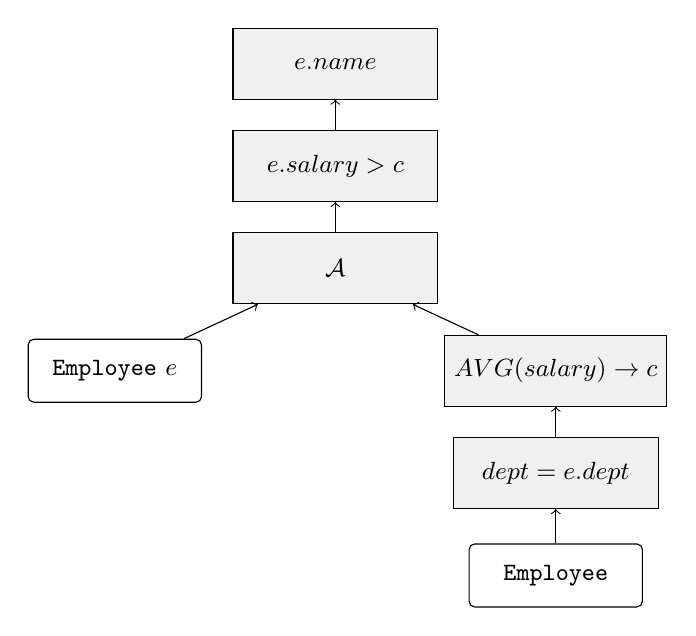
\begin{tikzpicture}[
    rel/.style={rectangle, draw, rounded corners=2pt, minimum width=2.2cm,
                minimum height=0.8cm, align=center, font=\small},
    op/.style={rectangle, draw, fill=gray!12, minimum width=2.6cm,
               minimum height=0.9cm, align=center, font=\small},
    level distance=1.15cm
]
    \node[op] (proj)  at (0, 6.5) {\(\Projection{e.\text{name}}{}\)};
    \node[op] (sel1)  at (0, 5.2) {\(\Sel{e.\text{salary} > c}{}\)};
    \node[op] (apply) at (0, 3.9) {\(\mathcal{A}\)};
    \node[rel] (emp1) at (-2.8, 2.6) {\texttt{Employee} \(e\)};
    \node[op] (agg)   at (2.8, 2.6) {\(\Agg{\varnothing}{\text{AVG}(\text{salary}) \to c}{}\)};
    \node[op] (sel2)  at (2.8, 1.3) {\(\Sel{\text{dept} = e.\text{dept}}{}\)};
    \node[rel] (emp2) at (2.8, 0) {\texttt{Employee}};

    \draw[->] (sel1)  -- (proj);
    \draw[->] (apply) -- (sel1);
    \draw[->] (emp1)  -- (apply);
    \draw[->] (agg)   -- (apply);
    \draw[->] (sel2)  -- (agg);
    \draw[->] (emp2)  -- (sel2);
\end{tikzpicture}
\caption{Дерево реляционной алгебры для запроса из
листинга~\ref{lst:correlated_subquery}.}%
\label{fig:correlated_subquery_tree}
\end{figure}

Преобразование в форму реляционной алгебры необходимо по нескольким причинам.
Во-первых, это позволяет использовать формализованный набор правил
эквивалентности, который позволяют оптимизатору корректно преобразовывать план
запроса без изменения семантики. Во-вторых, алгебраическое представление
позволяет единообразно обрабатывать различные синтаксические формы SQL-запросов,
порождающие одинаковые логические планы. Наконец, разделение на логические и
физические операторы позволяет оптимизатору независимо исследовать порядок
операций и алгоритмы их реализации.

\subsection{Поиск оптимального плана}

Эквивалентность планов, исследуемых в процессе поиска оптимального,
обеспечивается применением алгебраических тождеств, например ассоциативности и
коммутативности соединений. Правила эквивалентности реляционной алгебры подробно
рассматриваются в разделе~\ref{sec:transformation_rules}.

Оптимальность запроса принято оценивать с помощью функции стоимости
\(\mathrm{cost} \colon \mathcal{P}_L \to \mathbb{R}_{\ge 0}\)~\cite{Selinger1979},
где \(\mathcal{P}_{L}\) --- множество эквивалентных физических планов. Это
отображение оценивает затраты на исполнение плана исходя из конкретных
реализаций алгоритмов, а также основываясь на эвристиках и статистике о данных в
отношениях. Другими словами, цель оптимизатора состоит в том, чтобы для входного
запроса найти план \(P^* \in \mathcal{P}_L\), минимизирующий \(\mathrm{cost}\):
\[
  P^* = \arg\min_{P \in \mathcal{P}_L} \mathrm{cost}(P).
\]

Одной из подзадач в рамках построения оптимального плана является определение
порядка выполнения соединений. Благодаря правилам эквивалентости, таким как
ассоциативность и коммутативность соединения
(раздел~\ref{sec:transformation_rules}), одно и то же множество соединяемых
отношений допускает большое количество эквивалентных порядков вычисления.
Различные порядки имеют кардинально разные стоимости, ввиду особенностей
алгоритмов, реализующих соединение. Для \(n\) отношений количество таких
порядков выражается как
\(O(n! \cdot C_{n-1}) = O(\frac{(2n-2)!}{(n-1)!})\)~\cite{IntroToTheJoinOrderingProblem},
где \(C_k\) --- \(k\)-е число Каталана. Таким образом, пространство поиска
растет экспоненциально с увеличением числа соединяемых таблиц.

Поскольку полный перебор \(\mathcal{P}_L\) для достаточно больших \(n\)
невозможен, на практике речь идёт о поиске плана с приемлемо малой стоимостью в
определенном подмножестве пространства поиска. Именно эта задача и определяет
архитектуру современных оптимизаторов: расширяемое описание пространства поиска
через правила преобразования, эффективный алгоритм его исследования и
стоимостная модель, позволяющая отсекать заведомо неоптимальные ветви.

Выбор плана исполнения запроса может оказывать огромное влияние на объем
требуемых вычислительных ресурсов. В качестве примера оценим количество чтений
страниц с диска для различных физических операторов. Пусть имеется три
отношения: таблица \texttt{customer} с \(|C| = 10^5\) строк, таблица
\texttt{orders} с \(|O| = 10^7\) строк и таблица \texttt{lineitem} с
\(|L| = 5 \cdot 10^7\) строк. Размер страницы --- \(8\) КБ. В одну страницу
помещается \(100\) строк \texttt{customer}, \(80\) строк \texttt{orders} и
\(50\) строк \texttt{lineitem}. Соответственно, общее число страниц составляет
\(P_C = 10^3\), \(P_O = 1{,}25 \cdot 10^5\), \(P_L = 10^6\).

Для запроса из листинга~\ref{lst:join_query}
рассмотрим два альтернативных плана~\refImage{fig::join_plan_comparison}:
\begin{listing}
  \caption{Соединение \texttt{customer}, \texttt{orders} и \texttt{lineitem}.}
  \label{lst:join_query}
  \begin{minted}[style=bw, breaklines, frame=single, fontsize = \footnotesize, linenos=false, xleftmargin = 1.5em]{SQL}
  SELECT *
  FROM customer c
  JOIN orders o ON c.c_custkey = o.o_custkey
  JOIN lineitem l ON o.o_orderkey = l.l_orderkey
  \end{minted}
\end{listing}

\begin{figure}[!htb]\centering
\begin{tikzpicture}[
    rel/.style={rectangle, draw, rounded corners=2pt, minimum width=2.45cm,
                minimum height=0.8cm, align=center, font=\small},
    op/.style={rectangle, draw, fill=gray!12, minimum width=4.25cm,
               minimum height=1.2cm, align=center, font=\small}
]
    \node[op] (p1j2) at (-4.4, 2.9) {Hash Join\\\scriptsize \(10^6\) чтений};
    \node[op] (p1j1) at (-6.5, 1.2) {Hash Join\\\scriptsize \(1{,}26 \cdot 10^5\) чтений};
    \node[rel] (p1l) at (-2.3, 1.2) {\texttt{lineitem}};
    \node[rel] (p1c) at (-7.8, -0.3) {\texttt{customer}};
    \node[rel] (p1o) at (-4.4, -0.3) {\texttt{orders}};

    \draw[->] (p1j1) -- (p1j2);
    \draw[->] (p1l) -- (p1j2);
    \draw[->] (p1c) -- (p1j1);
    \draw[->] (p1o) -- (p1j1);
    \node[font=\small\bfseries] at (-4.4, 4.0) {План \(P_1\)};

    \node[op] (p2j2) at (4.4, 2.9) {Nested Loop Join\\\scriptsize \(1{,}25 \cdot 10^{14}\) чтений};
    \node[op] (p2j1) at (2.3, 1.2) {Nested Loop Join\\\scriptsize \(1{,}25 \cdot 10^8\) чтений};
    \node[rel] (p2l) at (6.5, 1.2) {\texttt{lineitem}};
    \node[rel] (p2c) at (1.0, -0.3) {\texttt{customer}};
    \node[rel] (p2o) at (4.4, -0.3) {\texttt{orders}};

    \draw[->] (p2j1) -- (p2j2);
    \draw[->] (p2l) -- (p2j2);
    \draw[->] (p2c) -- (p2j1);
    \draw[->] (p2o) -- (p2j1);
    \node[font=\small\bfseries] at (4.4, 4.0) {План \(P_2\)};
\end{tikzpicture}
\caption{Сравнение планов для запроса из листинга~\ref{lst:join_query}.}%
\label{fig::join_plan_comparison}
\end{figure}

\begin{itemize}
  \item План \(P_1\):
        \(\NJoin{(\NJoin{\texttt{customer}}{\texttt{orders}})}{\texttt{lineitem}}\)
        с реализацией обоих соединений через Hash Join, для чего сначала
        полностью считываются \(P_C + P_O = 1{,}26 \cdot 10^5\) страниц для
        построения хеш-таблицы, после чего промежуточный результат размером
        \(10^7\) строк соединяется с \texttt{lineitem}, требуя считывания ещё %
        \(P_L = 10^6\) страниц. В сумме --- порядка \(1{,}126 \cdot 10^6\)
        операций чтения с диска.
  \item План \(P_2\): тот же запрос, но реализованный как соединение с помощью
        вложенных циклов без использования индексов: для каждой строки
        \texttt{customer} полностью читается таблица \texttt{orders}, для каждой
        результирующей пары --- \texttt{lineitem}. Совокупный объём ввода-вывода
        оценивается величиной
        \(P_C \cdot P_O \cdot P_L \approx 1{,}25 \cdot 10^{14}\) операций
        чтения, что на восемь порядков превышает \(P_1\).
\end{itemize}

На еще одном примере запроса из листинга~\ref{lst:logical_transform_query}
рассмотрим влияние логических преобразований. Отношение \texttt{Emp} содержит
\(10{,}000\) кортежей, что эквивалентно \(1{,}000\) страницам. \texttt{Dept}
включает \(500\) записей и \(50\) страниц соответственно. Атрибут
\texttt{Emp.did} является внешним ключом к \texttt{Dept.did}, поэтому каждому
кортежу из \texttt{Dept} соответствует \(10{,}000 / 500 = 20\) из \texttt{Emp}.
Пусть на \texttt{Emp.did} и \texttt{Dept.dname} построены индексы, а в
промежуточную страницу помещается \(5\) кортежей.

\begin{listing}
  \caption{Пример запроса с проекцией, фильтрацией и соединением.}
  \label{lst:logical_transform_query}
  \begin{minted}[style=bw, breaklines, frame=single, fontsize = \footnotesize, linenos=false, xleftmargin = 1.5em]{SQL}
  SELECT DISTINCT ename
  FROM Emp E JOIN Dept D ON E.did = D.did
  WHERE D.dname = 'Toy'
  \end{minted}
\end{listing}

\begin{figure}[!htb]\centering
\begin{tikzpicture}[
    rel/.style={rectangle, draw, rounded corners=2pt, minimum width=2.0cm,
                minimum height=0.8cm, align=center, font=\small},
    op/.style={rectangle, draw, fill=gray!12, minimum width=4.5cm,
               minimum height=1.2cm, align=center, font=\small}
]
    \node[font=\small\bfseries] at (-3.5, 8.8) {План \(P_1\)};
    \node[op] (p1proj)  at (-3.5, 7.7) {\(\ProjectionOp{\texttt{ename}}\)};
    \node[op] (p1sig2)  at (-3.5, 6.2) {\(\SelOp{\texttt{dname}=\texttt{'Toy'}}\)};
    \node[op] (p1sig1)  at (-3.5, 4.7) {\(\SelOp{\texttt{Emp.did}=\texttt{Dept.did}}\)};
    \node[op] (p1cp)    at (-3.5, 3.2) {\(\CProd{\texttt{Emp}}{\texttt{Dept}}\)\\\scriptsize \(50{,}050\) чтений};
    \node[rel] (p1emp)  at (-5.2, 1.7) {\texttt{Emp}};
    \node[rel] (p1dept) at (-1.8, 1.7) {\texttt{Dept}};

    \draw[->] (p1emp)  -- (p1cp);
    \draw[->] (p1dept) -- (p1cp);
    \draw[->] (p1cp)   -- (p1sig1);
    \draw[->] (p1sig1) -- (p1sig2);
    \draw[->] (p1sig2) -- (p1proj);

    \node[font=\small\bfseries] at (3.5, 8.8) {План \(P_2\)};
    \node[op] (p2proj) at (3.5, 7.7) {\(\ProjectionOp{\texttt{ename}}\)};
    \node[op] (p2join) at (3.5, 5.5) {Index NL Join\\\(\texttt{Emp.did}=\texttt{Dept.did}\)\\\scriptsize \(23\) чтения};
    \node[rel] (p2emp) at (1.6, 3.5) {\texttt{Emp}};
    \node[op] (p2sig)  at (5.4, 3.5) {\(\SelOp{\texttt{dname}=\texttt{'Toy'}}\)\\\scriptsize \(3\) чтения};
    \node[rel] (p2dept) at (5.4, 1.8) {\texttt{Dept}};

    \draw[->] (p2emp)  -- (p2join);
    \draw[->] (p2sig)  -- (p2join);
    \draw[->] (p2join) -- (p2proj);
    \draw[->] (p2dept) -- (p2sig);
\end{tikzpicture}
\caption{Сравнение планов для запроса из
  листинга~\ref{lst:logical_transform_query}.}%
\label{fig::logical_transform_plans}
\end{figure}

Рассмотрим два плана~\refImage{fig::logical_transform_plans}:

\begin{itemize}
  \item План \(P_1\) соответствует прямому преобразованию запроса в реляционную
        алгебру, выполненному по алгоритму из раздела~\ref{sec:translation}.
        Если рассматривать стоимость исполнения такого плана в модели
        итераторов, то каждый оператор запрашивает у дочернего следующий кортеж
        через вызов \texttt{next()}, поэтому \(\sigma\) и~\(\pi\) работают в
        режиме конвейера и не инициируют обращений к диску. Вся стоимость
        ввода-вывода сосредоточена в операторе~\(\times\), реализованном через
        вложенные циклы с \texttt{Dept} в роли внешней таблицы: \texttt{Dept}
        читается один раз, а \texttt{Emp} перечитывается полностью для каждой
        страницы~\texttt{Dept}:
        \[
          50 + 50 \times 1{,}000 = 50{,}050 \text{ чтений.}
        \]

  \item План \(P_2\) является оптимизированным вариантом, где применено правило
        проталкивания предиката и декартово произведение заменено на соединение
        по предикату. Причем для доступа к таблице \texttt{Dept} применяется
        сканирование по индексу, что дает всего \(3\) чтения с диска. Соединение
        реализуется через вложенные циклы с использованием индекса, что в итоге дает:
        \[
          3 + (3 + 20) = 26 \text{ чтений.}
        \]
\end{itemize}

Оба приведенных примера наглядно демонстрируют, что оптимизатор отвечает за
принципиальную возможность исполнения сложных аналитических запросов за
приемлемое время. В первом случае разница между физическими планами составляет
восемь порядков: если \(P_1\) завершается за секунды, то наивный \(P_2\)
потребует десятков лет. Во втором случае даже единственное логическое
преобразование, в виде проталкивания предиката, снижает число чтений с диска в
\(1{,}900\) раз. Именно поэтому качественный оптимизатор является конкурентным
преимуществом и одной из самых важных частей СУБД.

\subsection{Обзор архитектур оптимизаторов}

System~R, разработанный в IBM Research в конце 1970-х годов~\cite{Selinger1979},
стал первым стоимостным оптимизатором. Его основная идея состоит в восходящем
динамическом программировании. Оптимизатор сначала выбирает лучшие методы
доступа к отдельным отношениям, затем строит лучшие планы для соединений из
двух, трех и большего числа отношений. Преимущество System~R заключается в
простоте и предсказуемости поиска, а также в учете стоимости ввода-вывода,
процессорных затрат и физических свойств операторов. Недостатки связаны с
ограниченной расширяемостью, ориентацией на левосторонние деревья соединений и
независимой оптимизацией вложенных подзапросов.

Volcano~\cite{GraefeMcKenna1993} развивает стоимостный подход System~R, но
делает оптимизатор расширяемым за счет правил и структуры Memo. В отличие от
System~R, пространство эквивалентных выражений задается не жестко встроенным
алгоритмом, а набором правил трансформации и реализации. Поиск выполняется
нисходящим динамическим программированием и может учитывать требуемые физические
свойства. Преимущество Volcano состоит в модульности и возможности добавлять
новые преобразования и операторы без переписывания всего оптимизатора. Основной
недостаток заключается в разделении поиска на фазу генерации и фазу стоимостного
анализа: предварительное раскрытие всех классов эквивалентности может приводить
к избыточной работе.

Cascades~\cite{Graefe1995} является развитием Volcano и сохраняет его ключевые
идеи: правила, Memo, физические свойства и стоимостный поиск. Главное отличие
Cascades состоит в том, что генерация альтернатив и стоимостная оптимизация не
разделяются на две независимые фазы, а чередуются через систему задач. Благодаря
этому оптимизатор может порождать только те альтернативы, которые нужны для
текущего поиска, раньше применять отсечения по стоимости и удобнее
распараллеливать независимые ветви. Недостатком Cascades является более сложная
реализация, так как требуется управлять состоянием групп, задачами поиска,
правилами и физическими свойствами.

\subsection{Архитектура Cascades}

В следующих разделах подробно рассматривается основные элементы архитектуры
оптимизаторов Cascades.

\subsubsection{Группы эквивалентности и выражения}

Группа представляет собой множество выражений, которые эквивалентны с
точки зрения логического результата. Например, для отношений \(A\), \(B\) и
\(C\) выражения \( \NJoin{A}{(\NJoin{B}{C})} ; \qquad{} \NJoin{(\NJoin{A}{B})}{C} \)
при выполнении условий ассоциативности соединения принадлежат одной группе,
поскольку возвращают одинаковый результат. Причем физические реализации этих
выражений могут отличаться, а стоимость может зависеть от кардинальности
промежуточных результатов.

Групповое выражение хранит оператор и ссылки на дочерние группы. Например,
выражение \(Join(G_1, G_2)\) не указывает конкретное дерево для левого и правого
входов, а ссылается на группы \(G_1\) и \(G_2\), каждая из которых может
содержать множество альтернатив. Поэтому одно групповое выражение кодирует
комбинацию многих конкретных деревьев, храня эту информацию компактно.

Memo является основной структурой данных для хранения групп эквивалентных
выражений в Cascades. Она выполняет функции устранения дублирующихся выражений,
хранит альтернативы, фиксирует результаты оптимизации под разными физическими
свойствами и является точкой синхронизации для задач поиска.

\begin{listing}
  \caption{Пример запроса.}
  \label{lst:query}
  \begin{minted}[style=bw, breaklines, frame=single, fontsize = \footnotesize, linenos=false, xleftmargin = 1.5em]{SQL}
    SELECT * FROM A JOIN B ON p_1 JOIN C ON p_2;
  \end{minted}
\end{listing}

На рисунке~\ref{fig:memo-structure} показан пример Memo для запроса из
листинга~\ref{lst:query}. Например, группа \(G_5\) представляет результат
соединения трех отношений, в ней находятся два логически эквивалентных выражения
с разной ассоциацией соединений и четыре физические реализации для них. Входными
данными для операторов являются группы, поэтому общие подвыражения не
дублируются.

При добавлении нового выражения Memo выполняет проверку на дубликаты. Если
выражение уже существует в некоторой группе, оно не добавляется повторно. В
случае, когда алгоритм в процессе работы обнаруживает эквивалентность двух ранее
различных групп, они эти группы объединяются в одну. При этом требуется
обновление ссылок и состояния правил.

\subsubsection{Алгоритм поиска}

Cascades организует оптимизацию как выполнение набора задач. Задача может
исследовать группу, исследовать выражение, применить правило, реализовать
логический оператор, оптимизировать дочернюю группу под заданное физическое
свойство или построить вспомогательный оператор для обеспечения свойства. Такой
подход позволяет гибко управлять порядком работы и откладывать дорогостоящие
действия до тех пор, пока они не станут необходимыми, а также разбивать поиск на
несколько этапов и распараллеливать исполнение независимых веток. При этом
однопоточные реализации хранят задачи в обычной очереди.

На рисунке~\ref{fig:cascades-tasks} показана схема взаимодействия задач в
оптимизаторе, а на
листингах~\ref{alg:cascades-search}-\ref{alg:cascades-search-2} приведен
псевдокод алгоритма поиска в архитектуре Cascades~\cite{DingNarasayya2024}.

Алгоритм реализуется в виде управляемого стеком поиска в пространстве
эквивалентных планов: сначала запускается оптимизация корневой группы,
\textsc{OptimizeGroup} в свою очередь исследует группу, а затем оптимизирует
каждое ее логическое выражение. Исследование выполняется через
\textsc{ExploreGroup} и \textsc{ExploreExpression}, которые сохраняют в Memo
новые логические выражения и группы с помощью правил преобразования. После этого
\textsc{OptimizeExpression} применяет правила реализации, превращая логические
выражения в физические. Для каждого физического варианта
\textsc{ApplyImplementation} проверяет локальную стоимость и передает план в
\textsc{OptimizeInputs}, где последовательно оптимизируются дочерние группы,
накапливается полная стоимость и обновляется информация о лучшем плане. Параметр
\texttt{limit} используется для отсечения заведомо дорогих вариантов.

\subsection{Правила трансформации и реализации}\label{sec:transformation_rules}

Правило в оптимизаторе Cascades состоит из образца, условия применимости и
алгоритма применения. Образец описывает форму логического выражения, к которому
может быть применено правило. Условие применимости проверяет дополнительные
требования: отсутствие внешних ссылок, тип соединения, сохранение семантики
\texttt{NULL}, совместимость свойств и другие ограничения.

Формально правило записывается в виде
\[
    r : \TransRule{pattern(e)}{condition(e)}{substitute(e)},
\]
где \(e\) --- исходное выражение, \(pattern\) --- структурный образец,
\(condition\) --- предикат применимости, \(substitute\) --- выражение-замена.
Для правил трансформации результатом применения является новое логическое
выражение в группе, а для правил реализации физическое выражение в той же
группе.

Правила трансформации задают эквивалентные преобразования логических выражений и
тем самым определяют пространство планов, исследуемое оптимизатором. Наиболее
важные из них представлены в таблице~\ref{tbl:transformation_rules}.

% TODO: может это вообще убрать? + нигде не описываю как выводятся свойства

\begin{Definition}
Null-отбрасывающим называется предикат, который при замене всех атрибутов
соответствующей стороны на \texttt{NULL} принимает значение, отличное от
\texttt{TRUE}.
\end{Definition}

\begin{Definition}
Конъюнкты \(\theta_1 \land \theta_2\) называются перераспределяемыми, если их
можно разбить на две группы \(\theta'_1\) и \(\theta'_2\) такие, что атрибуты
\(\theta'_2\) принадлежат \(attrs(S) \cup attrs(T)\), а конъюнкты с атрибутами
из \(attrs(R)\) остаются в \(\theta'_1\).
\end{Definition}

\begin{Definition}
Функция агрегации называется разделяемой, если она представима композицией
частичного агрегата и финального комбинатора. Например, \SUM{} раскладывается в
сумму частичных сумм, \AVG{} --- в пару \SUM{} и \COUNT{}.
\end{Definition}

Правила реализации переводят логические операторы в физические. Используемые в
настоящей работе правила собраны в таблице~\ref{tbl:implementation_rules}.

Физические свойства в Cascades обрабатываются через требуемые и предоставляемые
свойства. Если родительский оператор требует вход, отсортированный по атрибуту
\(a\), а выбранный дочерний план такого порядка не предоставляет, оптимизатор
может добавить обеспечивающий оператор \Sort.

Обеспечивающие операторы не изменяют логический результат, но меняют физические
свойства и увеличивают стоимость. Поэтому они рассматриваются наравне с другими
физическими альтернативами. Например, план с хеш-соединением и последующей
сортировкой может конкурировать с планом на основе соединения слиянием, которое
сохраняет порядок результата.

\subsubsection{Метод ветвей и границ}

% актуализировать: формулы, алгос и у меня другая селективность...

Метод ветвей и границ используется для сокращения пространства поиска и, как
следствие, неасимптотического улучшения скорости работы алгоритма. В контексте
Cascades ветвями являются альтернативные выражения и комбинации физических
реализаций дочерних групп, а границей является текущая лучшая стоимость плана
для заданной группы и требуемых физических свойств. Если нижняя оценка стоимости
частично построенного плана уже превышает текущую лучшую, дальнейшее
исследование по этой ветке не имеет смысла.

Пусть для группы \(G\) и требуемого свойства \(P\) уже найден план стоимости
\(C^*\). Рассматривается физическое выражение \(e\), имеющее локальную стоимость
\(C_{local}(e)\) и дочерние группы \(G_1, \ldots, G_k\). Если даже минимально
возможная оценка дочерних групп приводит к неравенству

\[
    C_{local}(e) + \sum_{i=1}^{k} LB(G_i, P_i) \geq C^*,
\]

то выражение \(e\) может быть отсечено. Здесь \(LB\) обозначает нижнюю границу
стоимости оптимизации дочерней группы под требуемым свойством \(P_i\). Чем
точнее нижняя граница, тем эффективнее отсечение.

На практике в качестве \(LB(G_i, P_i)\) принимается лучшая стоимость, найденная
для пары \((G_i, P_i)\) на текущий момент работы алгоритма. Поскольку
оптимизация группы является рекурсивным процессом, к моменту отсечения для
\((G_i, P_i)\) уже могут быть найдены некоторые планы, и их минимальная
стоимость служит нижней границей. Если же группа \(G_i\) под свойством \(P_i\)
ещё не рассматривалась, используется тривиальная граница \(LB = 0\), или, при
условии наличия минимальной стоимости на кортеж, можно принимать
\(LB(G_i, P_i) = |G_i| \cdot \mathit{minCostPerRow}\).

Требуемые свойства дочерних групп \(P_i\) определяются оператором выражения \(e\)
совместно с требованием родителя \(P\). Каждый физический оператор описывает, какие
свойства он ожидает от своих входов: например, оператор сортирующего слияния требует
упорядоченности обоих входов по соответствующим ключам, тогда как хеш-соединение не
предъявляет требований к порядку. Таким образом, при спуске по дереву поиска каждый
оператор транслирует глобальное требование \(P\) в конкретные требования \(P_1,
\ldots, P_k\) к своим дочерним группам.

\subsubsection{Оценка кардинальности}

Оценка кардинальности является процессом предсказания числа кортежей,
возвращаемых оператором.

Для выборки используется селективность предиката \(sel(p)\), после чего
кардинальность результата оценивается как

\[
    |\Sel{p}{R}| = |R| \cdot sel(p).
\]

Для соединения на основе предиката равенства независимых атрибутов часто
применяется эвристика:

\[
    |\InnerJoin{R}{R.a = S.b}{S}| \approx
    \frac{|R| \cdot |S|}{\max(NDV(R.a), NDV(S.b))},
\]

где \(NDV\) --- число различных значений атрибута. Такая оценка удобна, но может
быть грубой, если данные имеют корреляции, сильный перекос или сложные
зависимости между атрибутами. Экспериментальные исследования показывают, что
ошибки кардинальности часто являются одной из основных причин выбора неудачных
планов~\cite{leis2015good}.

Для повышения качества оценок используются гистограммы, статистики по
многоколоночным ключам, сведения об уникальности, функциональные зависимости,
ограничения на схему, а в современных исследованиях также модели машинного
обучения.

\subsubsection{Оценка стоимости}

Функция стоимости сопоставляет физическому плану численную оценку затрат на его
исполнение. Классическим считается представление стоимости в виде взвешенной
суммы операций чтения и записи страниц на диск, а также числа обработанных
кортежей и операций над ними~\cite{GraefeMcKenna1993,Graefe1995}:

\[
    Cost(p) = w_{io} \cdot IO(p) + w_{cpu} \cdot CPU(p).
\]

Коэффициенты \(w_{io}\), \(w_{cpu}\) зависят от конкретной аппаратной
конфигурации.

Стоимость является аддитивной и вычисляется рекурсивно по дереву физического
плана:

\[
    Cost(node) = LocalCost(node) + \sum_{child \in children(node)} Cost(child).
\]

Локальная стоимость оператора определяется его типом и кардинальностью его
входов. Пусть \(|R|\) --- кардинальность отношения \(R\), \(b\) --- блочный
фактор (число кортежей на странице), тогда \(P(R) = \lceil|R|/b\rceil\) ---
число страниц, занимаемых \(R\); \(c_\theta\) --- стоимость вычисления
предиката \(\theta\) на одной паре кортежей; \(\sigma_\theta\) ---
селективность предиката \(\theta\) (доля кортежей входа, удовлетворяющих
\(\theta\)); \(M\) --- число страниц буфера, доступных оператору. Формулы
локальной стоимости физических операторов приведены в
таблице~\ref{tbl:local-cost}.

\begin{longtable}{|l|c|c|}
  \caption{Локальная стоимость физических операторов.}\label{tbl:local-cost}\\
  \hline
  Оператор & \(IO(op)\) & \(CPU(op)\) \\
  \hline
  \endfirsthead
  \hline
  \endfoot

  \(\SeqScan(T)\) & \(P(T)\) & \(|T|\) \\ \hline
  \(\IndexScan(T, \theta)\) & \(\lceil \sigma_\theta \cdot P(T) \rceil\) & \(\sigma_\theta \cdot |T|\) \\ \hline
  \(\FilterOp(R, \theta)\) & \(0\) & \(|R| \cdot c_\theta\) \\ \hline
  \(\ProjOp(R)\) & \(0\) & \(|R|\) \\ \hline
  \(\NestedLoopJoin(L, R, \theta)\) & \(P(L) \cdot (1 + P(R))\) & \(|L| \cdot |R| \cdot c_\theta\) \\ \hline
  \(\NestedLoopCrossJoin(L, R)\) & \(P(L) \cdot (1 + P(R))\) & \(|L| \cdot |R|\) \\ \hline
  \(\HashJoin(L, R, \theta)\) & \(P(L) + P(R)\) & \(|L| + |R| \cdot (1 + c_\theta)\) \\ \hline
  \(\MergeJoin(L, R)\) & \(P(L) + P(R)\) & \(|L| + |R|\) \\ \hline
  \(\Sort(R)\) & \(2 P(R) \cdot \lceil \log_M P(R) \rceil\) & \(|R| \cdot \log_2 |R|\)
\end{longtable}

Для операторов \(\FilterOp\) и \(\ProjOp\) стоимость ввода-вывода равна \(0\), потому что это конвейерные операторы, которые не используют диск.

\subsection{Дифференциальный анализ физических планов}

Множество правил трансформации и реализации, используемых в
оптимизаторах запросов, изучено довольно хорошо и описано в
академической литературе. Вместе с тем условия активации правил
существенно различаются от системы к системе. Многие реализации
оптимизаторов упускают возможности для оптимизации из-за слишком
строгих условий активации правил или отсутствия определенных правил
в их наборе.

Данная проблема особенно актуальна при разработке нового оптимизатора: после
реализации базового набора правил возникает вопрос о полноте и корректности
этого набора по сравнению с устоявшимися и проверенными временем промышленными
системами. Такие системы аккумулировали обратную связь от пользователей и
уточняли условия активации своих правил в течение многих лет. Не имея такого
преимущества сложно добиться отличного качества построенных планов.

Решением может быть поиск несоответствий между поведением реализуемой системы и
внешней эталонной системы путем применения дифференциального анализа планов.

Первым шагом нужно сформировать несколько наборов данных, состоящих из схем
таблиц и их наполнения. Разные данные позволяют всесторонне исследовать правила
активации, потому что они зависят от кардинальности отношений, наличия индексов
и т.п.

Далее, по заданным схемам генерируются случайные SQL-запросы различной структуры
и сложности. Такой подход исключает тривиальные планы и приближает условия
работы оптимизатора к реальным нагрузкам при дальнейшем построении планов
запросов.

Следующим шагом сгенерированные запросы транспилируются в диалекты SQL целевых
промышленных СУБД. В качестве эталонных систем рассматриваются PostgreSQL,
DuckDB, Umbra и Microsoft SQL Server. Эти системы являются зрелыми, имеют
документированный формат вывода планов и представляют разные архитектурные
подходы. Затем для получения физических планов исполняется аналог
\texttt{EXPLAIN ANALYZE}.

Полученные физические планы промышленных СУБД конвертируются в формат
сериализованного плана разрабатываемого оптимизатора. Современные СУБД
предоставляют вывод планов в виде XML или JSON, что позволяет легко реализовать
их разбор. Для конвертации используется отображение между физическими
операторами разрабатываемой системы и операторами эталонной СУБД. Например,
\texttt{Hash Match} в SQL Server отображается в \HashJoin{} в разрабатываемой
системе, \texttt{Clustered Index Scan} --- в \IndexScan{} и так далее.
Восстановление предикатов, ключей соединения и выражений проекции выполняется
путем разбора соответствующих полей плана, причем не нужно поддерживать весь
синтаксис предикатов, так как генератор запросов и схемы данных ограничивают
множество допустимых выражений в планах.

Корректность конвертации выполняется по построению, но дополнительно проверяется
путем исполнения исходного плана на внешней системе и сконвертированного плана
на разрабатываемой системе с последующим сравнением полученных результатов при
фиксированной схеме и различных вариантах сгенерированных для нее данных.

Конвертированные планы сравниваются с планами, порождаемыми разрабатываемым
оптимизатором на исходных запросах, с целью определить, мог ли существующий
набор правил разрабатываемого оптимизатора породить план, эквивалентный плану
промышленной системы. Стоимостные модели и реализации операторов в разных СУБД
различаются, поэтому план, оптимальный для эталонной системы, не обязательно
будет оптимальным для разрабатываемой. По этоу причине сравнение направлено на
исследование полноты пространства поиска разрабатываемого оптимизатора, и не
предполагает сравнение эффективности планов.

Для корректности структурного сравнения необходимо полное исследование
пространства эквивалентных планов. Определение требуемых изменений лежит на
разработчике системы, поэтому найденный запрос и примеры планов сохраняются для
последующего анализа. В дальнейшем, полученные после конвертации ``эталонные''
планы можно использовать как тесты для оптимизатора, которые будут успешно
выполняться после уточнения соответвующих правил активации.

В случае невозможности построить ``эталонный'' план разрабатываемым
оптимизатором, предлагается искать ближайший план, т.е. план из пространства
поиска разрабатываемого оптимизатора, максимально близкий к плану промышленной
системы. При этом метрика расстояния между планами может быть определена как
расстояние редактирования деревьев.

Анализ ближайшего плана может помочь упростить выявление трансформаций, которые
разрабатываемый план по какой-то причине не применил.

Предлагаемый метод дифференциального анализа применим для сравнения как с
проприетарными системами, так и с СУБД с открытым исходным кодом, позволяя
уточнять условия применения правил.

Систематическое применение этого подхода позволяет построить итеративный процесс
совершенствования оптимизатора:

\begin{itemize}
  \item генерация запросов;
  \item запуск и сбор планов;
  \item приведение к единому виду, сравнение и выявление расхождений;
  \item добавление или корректировка правил;
  \item повторное сравнение.
\end{itemize}

Таким образом, дифференциальный анализ обеспечивает управляемое и измеримое
улучшение качества оптимизатора и позволяет новым или открытым оптимизаторам
быстрее достигать качества устоявшихся промышленных оптимизаторов.

% {\color{red} TODO: описать как нормализовать и т.п.}

\section{Конструкторская часть}

В рамках данной работы был разработан оптимизатор запросов для модельной
реляционной СУБД.

Структурно реализация модельной СУБД состоит из следующих модулей:
\begin{itemize}
  \item модуль синтаксического анализа SQL-запросов;
  \item модуль построения логического представления запроса;
  \item модуль стоимостной оптимизации на основе структуры Memo;
  \item подсистема физического хранения на основе статических CSV-таблиц;
  \item модуль исполнения физических операторов.
\end{itemize}

Основой для проектирования оптимизатора была выбрана архитектура Cascades. В ней
пространство допустимых планов формируется с помощью набора правил
преобразования и хранится в структуре Memo. Эта структура объединяет логически
эквивалентные выражения в группы, что позволяет избежать повторного рассмотрения
одинаковых поддеревьев. Поиск оптимального физического плана выполняется с учетом
стоимостной модели и требуемых свойств результата, например порядка сортировки.

Данная архитектура была выбрана по причине ее модульности и расширяемости.
Добавление новых логических преобразований и физических операторов выполняется
путем реализации отдельных правил и не требует изменения основного алгоритма
поиска. Это также удобно для итеративного процесса разработки, предполагающего
постепенное улучшение качества итоговых планов путем уточнения и расширения
пространства поиска.

\subsection{Модули синтаксического анализа и построения логического представления}

Модуль синтаксического анализа SQL-запросов отвечает за лексический и
синтаксический разбор поступающих на вход SQL-запросов. В качестве основы для
грамматики выбран диалект PostgreSQL, так как он широко используется на практике
и имеет открытый исходный код. Использование готовой грамматики из официального
репозитория~\cite{PostgresBisonGrammar} гарантирует совместимость.

В рамках работы поддерживается подмножество диалекта PostgreSQL, достаточное для
исследования оптимизации запросов на чтение данных. В него входят операторы
\SELECT{} с предложениями \FROM, \WHERE, \GROUPBY{} и \ORDERBY{}, выбор всех
столбцов или списка выражений, псевдонимы, соединения \JOIN, \sqlkw{INNER JOIN},
\sqlkw{LEFT JOIN}, \sqlkw{RIGHT JOIN}, \sqlkw{FULL JOIN} с условием \sqlkw{ON},
а также \sqlkw{CROSS JOIN}. Для группировки поддерживаются обычные выражения в
\GROUPBY{} и агрегатные функции \SUM{}, \COUNT{} и \sqlkw{COUNT(*)}. Сортировка
результата задается через \ORDERBY{} по ссылкам на столбцы в прямом или обратном
порядке.

Поддерживаемые скалярные выражения включают ссылки на столбцы, целочисленные
константы, строковые литералы в одинарных кавычках, значения \sqlkw{NULL},
\sqlkw{TRUE}, \sqlkw{FALSE} и \sqlkw{UNKNOWN}, арифметические операции сложения,
вычитания, умножения, деления, остатка от деления и возведения в степень, а
также унарный минус. В предикатах поддерживаются операции сравнения, логические
связки \sqlkw{AND}, \sqlkw{OR} и \sqlkw{NOT}, проверки \sqlkw{IS NULL},
\sqlkw{IS TRUE}, \sqlkw{IS FALSE}, \sqlkw{IS UNKNOWN}, условия \sqlkw{BETWEEN} и
\sqlkw{IN} со списком значений. Такое подмножество покрывает основные
конструкции, влияющие на построение логического плана: проекцию, фильтрацию,
соединение, агрегацию и требование сортировки результата.

Модуль построения логического представления запроса отвечает за преобразование
результата синтаксического анализа во внутреннее представление, пригодное для
оптимизации. В качестве такого представления решено использовать дерево
операторов реляционной алгебры. Этот подход является общепринятым и позволяет
отделить особенности синтаксиса SQL от последующих этапов обработки запроса, а
также выполнять оптимизацию над ограниченным набором формализованных операций:
фильтрацией, проекцией, соединением, агрегацией и сортировкой.

\subsection{Модули физического хранения и исполнения}

Подсистема физического хранения отвечает за предоставление модулю исполнения
табличных данных. Для хранения выбраны статические таблицы в формате CSV.
Использование простого текстового формата позволяет сосредоточиться на
проектировании оптимизатора и не усложнять прототип реализацией транзакций,
индексов, буферного кэша и управления дисковыми страницами. Кроме того,
CSV-файлы удобно создавать, изменять и использовать при проведении тестов.

Данные хранятся в одной директории, где каждому отношению соответствует
файл с CSV-таблицей. Название файла совпадает с названием отношения.
Первая строка CSV-файла содержит описание атрибутов и их типов,
последующие строки содержат кортежи отношения.

Дополнительно предусмотрена поддержка индексов. Индекс представляет собой
отсортированный бинарный файл, содержащий целочисленные ключи и смещения
соответствующих строк в CSV-файле. Использование смещений позволяет
извлекать подходящие кортежи без полного сканирования отношения.

Модуль исполнения физических операторов отвечает за выполнение выбранного
оптимизатором плана и формирование результата запроса. Физический план решено
представлять в виде дерева операторов с единым интерфейсом взаимодействия.
Каждый оператор получает данные от дочерних узлов, выполняет определенное
преобразование и передает результат вышестоящему оператору. Такой подход
обеспечивает модульность подсистемы исполнения и позволяет добавлять новые
физические операторы независимо от уже реализованных.

\subsection{Модуль стоимостной оптимизации планов}

Модуль стоимостной оптимизации планов принимает на вход логическое представление
запроса и строит физический план исполнения с минимальной оцененной стоимостью.
В качестве основы выбран подход Cascades. Исходное дерево логических операторов
помещается в структуру Memo, после чего оптимизатор постепенно расширяет
пространство поиска с помощью правил преобразования и правил реализации. Такой
подход позволяет не хранить каждое дерево плана отдельно, а компактно
представлять множество эквивалентных вариантов через группы Memo.

Каждая группа Memo соответствует множеству логически эквивалентных выражений,
то есть выражений, возвращающих один и тот же результат. Логические выражения
содержат ссылки на дочерние группы, поэтому один узел может представлять сразу
несколько вариантов построения поддерева. В процессе оптимизации в группы
добавляются как новые логические выражения, полученные правилами
трансформации, так и физические выражения, полученные правилами реализации.

Правило трансформации создает новое логическое выражение и добавляет его в
ту же группу Memo, что и исходное выражение. Следовательно, правило должно
сохранять семантику запроса. Правило реализации создает физическое выражение,
которое может быть передано модулю исполнения.

Реализованы следующие трансформационные правила:
\begin{itemize}
  \item коммутативность соединения;
  \item ассоциативность соединения;
  \item разбиение конъюнкции на последовательность фильтров;
  \item объединение последовательных фильтров;
  \item проталкивание фильтра через проекцию;
  \item проталкивание фильтра во входы соединения;
  \item преобразование выражения \verb|IN| в цепочку сравнений.
\end{itemize}

И следующие правила реализации:
\begin{itemize}
  \item последовательное сканирование таблицы;
  \item фильтрация;
  \item проекция;
  \item хэш-агрегация;
  \item потоковая агрегация;
  \item декартово произведение вложенными циклами;
  \item соединение вложенными циклами;
  \item хеш-соединение;
  \item соединение слиянием.
\end{itemize}

Данный набор правил все основные алгоритмы, реализующие операторы реляционной
алгебры, и включает самые важные правила трансформации. Также более полное
покрытие правилами реализации хорошо подходит для демонтрации возможностей
дифференциального сравнения планов для последующего расширения покрытия
правилами трансформации.

Выбор лучшего плана выполняется на основе стоимостной модели. Стоимость
физического оператора рассчитывается с учетом оценок кардинальности входных и
выходных групп. Формулы для вычисления стоимости откалиброваны по результатам
бенчмарков и представлены в табилце~\ref{tbl:cost-model-coefficients}.
Кардинальность базовых отношений берется из описания входных таблиц, а для
фильтров, соединений, агрегаций и проекций оценивается эвристически. Чтобы
сократить перебор, оптимизатор использует метод ветвей и границ. Если локальная
стоимость или нижняя оценка стоимости поддерева уже превышает текущий лучший
результат, соответствующая ветвь пространства поиска не рассматривается дальше.

Для оценки кардинальности промежуточных результатов используется коэффициент
селективности \(sel(p)\), показывающий долю кортежей, удовлетворяющих предикату
\(p\). Используемые формулы приведены в таблице~\ref{tbl:selectivity-model}.

Такие формулы выбраны как простая эвристическая модель, не требующая гистограмм,
сведений о количестве различных значений и статистик корреляции между
атрибутами. Равенство атрибута константе считается достаточно селективным,
поэтому ему сопоставляется коэффициент \(0{,}10\). Диапазонные и неизвестные
условия оцениваются нейтральным коэффициентом \(0{,}50\), так как без статистики
нельзя надежно определить, какую часть отношения они оставят. Для \sqlkw{IN}
используется сумма селективностей отдельных равенств с верхней границей
\(0{,}50\), чтобы длинный список значений не делал оценку слишком оптимистичной.

Формулы для \sqlkw{AND}, \sqlkw{OR} и \sqlkw{NOT} основаны на предположении
независимости предикатов. Для эквисоединения двух атрибутов используется оценка
\(1 / \max(n_l, n_r)\), соответствующая типичному случаю соединения по ключу или
внешнему ключу, размер результата в таком случае оказывается сопоставим с
размером большего входа, а не с полным декартовым произведением. Для неизвестных
условий соединения применяется селективность \(1\), чтобы не занижать стоимость
плана при отсутствии надежной информации.

Отдельно учитываются физические свойства результата. В данной работе таким
свойством является порядок строк, требуемый предложением \ORDERBY{}. Если
выбранный план не обеспечивает требуемую сортировку, оптимизатор может добавить
обеспечивающий физический оператор сортировки и сравнить его стоимость с
другими альтернативами. Результатом работы модуля является дерево физических
операторов, которое передается в модуль исполнения.

\section{Технологическая часть}

Программа написана на языке C++ с использованием стандарта C++23. Этот язык
популярен в сфере разработки СУБД, являясь достаточно низкоуровневым и
производительным, но в то же время удобным для реализации больших систем. Для
сборки применяется CMake и его встроенные средства для зависимостей в виде
библиотек на C++. Окружение для разработки описывается декларативно и
воспроизводимо при помощи функционального доменно-специфичного языка \verb|nix|
для соответствующего пакетного менеджера.

Для синтаксического анализа выбран генератор парсеров ANTLR4, ввиду простоты и
удобства в использовании. Асинхронное взаимодействие физических операторов
построено на Boost.Asio, по причине совместимости со встроенными в язык
корутинами и понятной модели асинхронности. Для тестирования корректности и
производительности используется Google Tests, Google Benchmarks и pytest.

\subsection{Модуль синтаксического анализа}

Для реализации парсера был выбран ANTLR4, ввиду его удобства и возможности
генерировать лексические и синтаксические анализаторы под практически любой язык
программирования.

Грамматика PostgreSQL была взята из официального репозитория проекта
ANTLR4~\cite{Antlr4PostgreSQL}. Она была портирована автоматически из грамматики
для Bison~\cite{PostgresBisonGrammar} из официального репозитория Postgres,
поэтому является наиболее полной из существующих.

ANTLR4 генерирует несколько файлов на C++, в том числе лексический и
синтаксический анализаторы, а также класс \verb|Visitor| для обхода дерева
разбора. Для интересующих конструкций SQL переопределены методы посещения узлов
грамматики. Например, предложение \WHERE{} преобразуется в логический оператор
фильтрации, список выражений после \SELECT{} преобразуется в проекцию, а список
таблиц после \FROM{} --- в дерево соединений.

Результатом работы парсера является структура \texttt{ParsedQuery}. Она содержит
логический оператор верхнего уровня и необязательное требование к порядку строк
для \ORDERBY{}. Логические операторы и скалярные выражения представлены
алгебраическими типами на основе \texttt{std::variant}. В них входят операторы
таблицы, фильтрации, проекции, агрегации, соединения, ссылки на атрибуты,
константы и арифметические выражения~\refAlgo{lst:logical}.

\begin{listing}[H]
  \caption{Объявление типов для операторов реляционной алегебры и выражений.}
  \label{lst:logical}
  \begin{minted}[style=bw, breaklines, frame=single, fontsize = \footnotesize, linenos=false, xleftmargin = 1.5em]{C++}
using Operator = std::variant<Table, Projection, Filter, Aggregation, CrossJoin, Join>;

using Expression = std::variant<BinaryExpression, Attribute, IntConst, StringConst, UnaryExpression, InExpression, AggregateExpression, Literal>;

struct Projection {
    std::vector<Expression> expressions;
    std::shared_ptr<Operator> source;
    std::vector<std::optional<std::string>> aliases;

    bool operator==(const Projection& other) const;
};
  \end{minted}
\end{listing}

Выражения хранятся в алгебраическом типе \verb|Expression|, реализованном
аналогично \verb|Operator|.

Функция \verb|GetAST| внутри строит абстрактное синтаксическое дерево и обходит
его с помощью \verb|Visitor|, который и генерирует представление запроса в виде
дерева из \verb|Operator|.

Дополнительно реализована визуализация дерева из операторов реляционной алгебры
в формате Graphviz с помощью функции \verb|GetDotRepresentation|.

\subsection{Модуль оптимизации запросов}

Модуль оптимизации запросов отвечает за преобразование логического дерева
операторов в физический план исполнения с минимальной оцененной стоимостью.
Пространство исследуемых эквивалентных планов эффективно хранится в структуре
Memo и расширяется с помощью добавления новых правил. Поиск выполняется сверху
вниз с использованием стоимостной модели, физических свойств и метода ветвей и
границ.

Центральное место в оптимизаторе занимает структура Memo, которая хранит группы
логически эквивалентных выражений. Выражения из одной группы возвращают
одинаковый результат. Например, $A \Join B$ и $B \Join A$ являются
эквивалентными.

Дочерние узлы выражения ссылаются не на конкретные операторы, а на группы.
Благодаря этому одно выражение компактно представляет множество деревьев.
Объявления классов \verb|Memo| и \verb|Group| приведены в
листинге~\ref{lst:memo}.

\begin{listing}[H]
  \caption{Основные элементы структуры Memo.}
  \label{lst:memo}
  \begin{minted}[style=bw, breaklines, frame=single,
    fontsize=\footnotesize, linenos=false, xleftmargin=1.5em]{cpp}
class Memo {
public:
  utils::NotNull<LogicalExpr*> AddGroup(LogicalOperator op);
  utils::NotNull<LogicalExpr*> AddLogicalExprToGroup(
      utils::NotNull<Group*> group, LogicalOperator op);
  utils::NotNull<LogicalExpr*> Populate(const Operator& op);

private:
  std::deque<Group> groups_;
  std::unordered_map<std::string, LogicalExpr*> expr_index_;
};

class Group {
public:
  utils::NotNull<LogicalExpr*> AddLogicalExpr(LogicalOperator op);
  utils::NotNull<PhysicalExpr*> AddPhysicalExpr(
      PhysicalOperator op, bool is_enforcer = false);

  LogicalExprs GetLogicalExprs();
  PhysicalExprs GetPhysicalExprs();
};
  \end{minted}
\end{listing}

Метод \verb|Memo::Populate| рекурсивно обходит исходное логическое дерево и
создает первоначальные группы. Для предотвращения повторного добавления
выражений используется отображение \verb|expr_index_|. Ключ строится из типа
оператора, его параметров и идентификаторов дочерних групп. Таким образом,
одинаковые выражения добавляются в Memo только один раз.

Каждая группа содержит логические и физические выражения. Логические выражения
описывают семантику запроса, а физические выражения определяют конкретный способ
исполнения. Например, логическому соединению могут соответствовать физические
операторы соединения вложенными циклами и хеш-соединения.

\subsubsection{Правила трансформации и реализации}

Расширение пространства поиска выполняется с помощью правил. Реализовано два
типа правил: трансформационные и реализационные. % Их интерфейсы приведены в
% листинге~\ref{lst:optimizer-rules}.
Правила реализуют единый интерфейс, состоящий из условия применимости и метода
для применения правила. Условие применимости выполняет быструю структурную
проверку по дереву выражений в Memo. Метод применения правила порождает
необходимые новые группы и результирующее логическое или физическое выражение. В
качестве примера в листинге~\ref{lst:join-commutativity} приведена реализация
правила коммутативности соединений.

% \begin{listing}[H]
%   \caption{Интерфейсы правил оптимизации.}
%   \label{lst:optimizer-rules}
%   \begin{minted}[style=bw, breaklines, frame=single,
%     fontsize=\footnotesize, linenos=false, xleftmargin=1.5em]{cpp}
% class TransformationRule {
% public:
%   virtual bool IsApplicable(utils::NotNull<LogicalExpr*> expr) = 0;
%   utils::NotNull<LogicalExpr*> Apply(
%       utils::NotNull<LogicalExpr*> expr, Memo& memo);
% private:
%   virtual LogicalOperator ApplyImpl(
%       utils::NotNull<LogicalExpr*> expr, Memo& memo) = 0;
% };
% class ImplementationRule {
% public:
%   virtual bool IsApplicable(utils::NotNull<LogicalExpr*> expr) = 0;
%   virtual utils::NotNull<PhysicalExpr*> Apply(
%       utils::NotNull<LogicalExpr*> expr, Memo& memo) = 0;
% };
%   \end{minted}
% \end{listing}

Для каждого выражения хранится информация о ранее примененных правилах. Это
предотвращает повторное выполнение одного правила над одним выражением и
ограничивает образование циклов при заполнении Memo.

\subsubsection{Стоимостная модель}

Стоимость физического плана зависит от количества обрабатываемых кортежей. Для
получения этой величины используется класс \verb|CardinalityEstimates|. Оценка
кардинальности вычисляется для группы Memo и кэшируется.

Стоимость плана вычисляется как сумма локальных стоимостей физических
операторов. Фрагмент реализации стоимостной модели приведен в
листинге~\ref{lst:optimizer-cost}.

\subsubsection{Алгоритм поиска}

Класс \verb|Optimizer| реализует алгоритм поиска. При создании объекта исходное
логическое дерево помещается в Memo. Поиск запускается для корневой группы и
требуемых физических свойств результата.

Алгоритм использует стек отложенных задач. Это позволяет разделить процесс на
небольшие операции: исследование группы, применение правила, оптимизацию
физического выражения и обработку его дочерних узлов. Основной метод оптимизации
группы приведен в листинге~\ref{lst:optimize-group}.

Если группа еще не исследована, в стек добавляются две задачи. Первая расширяет
группу с помощью правил, вторая повторно запускает ее оптимизацию после
расширения. Если группа уже исследована, для каждого физического выражения
вычисляется полная стоимость с учетом дочерних групп.

Для каждой пары из группы и требуемого набора свойств хранится лучший найденный
вариант. Ключ такого варианта представлен структурой
\verb|WinnerKey|~\refAlgo{lst:winner-key}. Хранение победителя отдельно для каждого
набора свойств необходимо, поскольку самый дешевый неотсортированный план может
отличаться от самого дешевого плана, удовлетворяющего требованию
\verb|ORDER BY|.

\begin{listing}[H]
  \caption{Ключ для хранения лучшего плана по группе и свойствам.}
  \label{lst:winner-key}
  \begin{minted}[style=bw, breaklines, frame=single,
    fontsize=\footnotesize, linenos=false, xleftmargin=1.5em]{cpp}
struct WinnerKey {
  Group* group;
  PropertySet required;
};
\end{minted}
\end{listing}

Дочерние группы физического выражения оптимизируются последовательно. После
получения победителя дочерней группы его стоимость прибавляется к накопленной
стоимости. Если все дочерние группы обработаны, проверяются выходные свойства
плана. Затем найденный вариант может стать новым лучшим планом.

\subsubsection{Метод ветвей и границ}

Полный перебор пространства планов быстро становится непрактичным при
увеличении количества соединяемых таблиц. Для сокращения перебора используется
метод ветвей и границ.

Для каждой группы вычисляется нижняя граница стоимости. Она равна минимальной
сумме нижней оценки локального оператора и нижних оценок дочерних групп.
Например, для логического соединения выбирается минимум между стоимостью
хеш-соединения и стоимостью соединения вложенными циклами:
\[
  LB_{\text{join}} =
  \min(69(N_l + N_r), 70N_lN_r).
\]

Если нижняя граница не меньше стоимости уже известного решения, исследование
ветви прекращается. Фрагмент реализации приведен в
листинге~\ref{lst:lower-bound}.

\begin{listing}[H]
  \caption{Вычисление нижней границы стоимости группы.}
  \label{lst:lower-bound}
  \begin{minted}[style=bw, breaklines, frame=single,
    fontsize=\footnotesize, linenos=false, xleftmargin=1.5em]{cpp}
int64_t Optimizer::LowerBoundCost(Group* group) {
  if (auto it = lower_bounds_.find(group);
      it != lower_bounds_.end()) {
    return it->second;
  }
  int64_t best = std::numeric_limits<int64_t>::max();
  for (auto expr : group->GetLogicalExprs()) {
    int64_t cost = LowerBoundLocalCost(expr, cardinality_);
    for (auto child : GetChildren(expr)) {
      cost += LowerBoundCost(child);
    }
    best = std::min(best, cost);
  }
  lower_bounds_[group] = best;
  return best;
}
  \end{minted}
\end{listing}

Метод \verb|OptimizeInputs| также уменьшает границу для очередного дочернего
узла. Из общей допустимой стоимости вычитаются уже накопленная стоимость и
нижние оценки еще не обработанных дочерних групп. Благодаря этому заведомо
неоптимальные ветви отбрасываются до построения полного плана.

% Для исследовательских задач предусмотрен метод \verb|OptimizeExhaustive|. Он
% запускает тот же алгоритм без ограничения стоимости и используется при проверке
% достижимости внешних физических планов.

\subsubsection{Физические свойства}

Некоторые требования к результату нельзя выразить только стоимостью. Например,
конструкция \verb|ORDER BY| требует от результата определенного порядка
кортежей. Для представления таких требований используется класс
\verb|PropertySet|.

Например, порядок сортировки считается удовлетворяющим требованию, если
требуемые ключи являются префиксом фактически полученного порядка. Таким образом
сортировка по $(a, b)$ удовлетворяет требованию сортировки по $a$.

Некоторые операторы сохраняют порядок дочернего узла. Фильтрация и проекция
сохраняют свойства входа. Соединение вложенными циклами сохраняет свойства
левого входа. Хеш-соединение и агрегация не гарантируют сохранение порядка.

Если подходящий план не найден, оптимизатор пытается добавить обеспечивающий
оператор. Для сортировки используется класс \verb|SortEnforcer|. Он проверяет
наличие требуемых атрибутов в схеме группы и создает физический оператор
сортировки.

\begin{listing}[H]
  \caption{Добавление оператора сортировки для обеспечения свойства.}
  \label{lst:sort-enforcer}
  \begin{minted}[style=bw, breaklines, frame=single,
    fontsize=\footnotesize, linenos=false, xleftmargin=1.5em]{cpp}
std::optional<PhysicalOperator> SortEnforcer::TryBuild(
    utils::NotNull<Group*> group,
    const PropertySet& required,
    SchemaCatalog& schema) const {
  const auto* sort = required.Get<SortProperty>();
  if (!sort) return std::nullopt;
  if (!ContainsRequiredKeys(schema.GetSchema(group),
                            sort->order)) {
    return std::nullopt;
  }
  return physical::Sort{group, sort->order};
}
  \end{minted}
\end{listing}

\subsubsection{Формирование физического плана}

После завершения поиска метод \verb|BuildOptimalPlan| рекурсивно восстанавливает
итоговое дерево физических операторов. Для каждой группы выбирается сохраненный
лучший план с учетом требуемых свойств. Затем аналогичным образом
восстанавливаются планы дочерних групп.

Результатом работы оптимизатора является объект \verb|PhysicalPlanNode|, который
не зависит от структуры Memo. Он может быть сериализован для анализа или передан
модулю исполнения запросов.

Таким образом, модуль оптимизации разделяет представление пространства планов,
правила его расширения, стоимостную модель и алгоритм поиска. Такая организация
позволяет добавлять новые правила и физические операторы без изменения основной
логики оптимизатора.

\subsection{Модуль физического хранения данных}

Для чтения таблиц реализован класс \verb|CsvDirSequentialScanner|. Он выполняет
последовательное сканирование CSV-файла и передает прочитанные кортежи модулю
исполнения физических операторов.

Список доступных индексов задается в файле \verb|indexes.meta|,
расположенном в директории с данными. Каждая строка файла содержит
название отношения, название индексируемого атрибута, тип индекса и имя
бинарного файла~\refAlgo{lst:meta}.

\begin{listing}[H]
  \caption{Пример файла с метаданными о доступных индексах.}
  \label{lst:meta}
\begin{minted}[style=bw, breaklines, frame=single, fontsize = \footnotesize, linenos=false, xleftmargin = 1.5em]{text}
users id sorted users.id.sorted.idx
\end{minted}
\end{listing}

Для чтения данных с использованием индекса реализован класс
\verb|CsvDirIndexedScanner|. Если указанный в метаданных бинарный файл
отсутствует, индекс строится при первом обращении к таблице. Для поиска
диапазона подходящих ключей используется упорядоченность записей индекса.

Поддерживаются индексы только для целочисленных атрибутов. Индексное
сканирование применяется для предикатов сравнения атрибута с целочисленной
константой. Из возможных операций доступно равенство, строгое и нестрогое
сравнение. После чтения найденных строк дополнительно вычисляется исходный
предикат, что обеспечивает корректную обработку составных условий.

\subsection{Модуль исполнения физических планов}

За исполнение запросов отвечает класс \verb|Executor|~\refAlgo{lst:executor}. Он
получает физический план, запускает исполнение его операторов и формирует
результирующее отношение. Физический план представлен деревом объектов типа
\verb|PhysicalPlanNode|. Для каждого типа узла предусмотрена отдельная функция
исполнения реализующая единый интерфейс и исполняющаяся независимо.

\begin{listing}[H]
  \caption{Основные элементы объявления класса Executor.}
  \label{lst:executor}
  \begin{minted}[style=bw, breaklines, frame=single, fontsize = \footnotesize, linenos=false, xleftmargin = 1.5em]{C++}
template <typename ExpressionExecutor = InterpretedExpressionExecutor>
class Executor {
public:
  Executor(SequentialScan seq_scan,
            IndexScan index_scan,
            boost::asio::any_io_executor executor);
  boost::asio::awaitable<Result<Relation>>
  Execute(const PhysicalPlanNode& op);
private:
  SequentialScan sequential_scan_;
  IndexScan index_scan_;
  ExpressionExecutor expression_executor_;
};
  \end{minted}
\end{listing}

Класс параметризуется интерфейсами \verb|SequentialScan|, \verb|IndexScan| и
\verb|ExpressionExecutor|. Первые два интерфейса отделяют исполнение физического
плана от конкретного способа хранения данных. \verb|SequentialScan| выполняет
полное чтение таблицы, а \verb|IndexScan| получает дополнительный предикат и
извлекает строки с использованием индекса. Благодаря этому исполнитель не
зависит от формата CSV-файлов и устройства индексных структур.

Параметр \verb|ExpressionExecutor| определяет способ вычисления скалярных
выражений. Реализованы стратегии для интерпретации выражений и для
JIT-компиляции. По умолчанию используется интерпретируемый вариант.

Значения атрибутов представлены структурой \verb|Value|. Она содержит признак
\verb|NULL| и значение одного из поддерживаемых типов: целого числа, логического
значения или идентификатора строки. Исходное значение для строк сохраняется в
пул, а в кортеже хранится числовой идентификатор строки. Кортеж представлен
вектором значений, а отношение состоит из описания атрибутов и списка кортежей.

Коммуникация между физическими операторами осуществляется с помощью асинхронных
каналов. Используются два типа каналов: \verb|AttributesInfoChannel| для
однократной передачи схемы отношения и \verb|TuplesChannel| для передачи данных.
Кортежи передаются векторами. Это уменьшает число операций синхронизации и
позволяет потоковым операторам начинать обработку до полного завершения дочерних
узлов плана.

Для реализации каналов используется
\verb|boost::asio::experimental::concurrent_channel|. Данный класс обеспечивает
потокобезопасность, буферизацию, асинхронную передачу данных и совместимость с
корутинами. Такой подход позволяет единообразно организовать взаимодействие
между операторами независимо от конкретных алгоритмов для их реализации.

\subsection{Руководство пользователя}

Для сборки программы требуются CMake, компилятор C++ с поддержкой C++23, LLVM,
ANTLR4 и библиотеки Boost. Дополнительно требуется Python, pytest и Docker. В
репозитории присутствует файл \texttt{flake.nix}, описывающий необходимые
зависимости, поэтому в системе с пакетным менеджером Nix рекомендуется открыть
окружение при помощи команды \verb|nix develop|.

Все команды далее выполняются из корневого каталога проекта.

\subsubsection{Сборка программы}

Для выполнения конфигурации и сборки следует запустить команды на листинге~\ref{lst:build}.

\begin{listing}[H]
  \caption{Конфигурация и сборка проекта.}
  \label{lst:build}
  \begin{minted}[style=bw, breaklines, frame=single, fontsize=\footnotesize, linenos=false, xleftmargin=1.5em]{bash}
cmake -S . -B build -DCMAKE_BUILD_TYPE=Release
cmake --build build -- -j 6
  \end{minted}
\end{listing}

После успешной сборки исполняемый файл находится по пути
\texttt{build/bin/sql}. Для повторной сборки также можно использовать цель
\texttt{make build}.

\subsubsection{Запуск программы}

Пользователь должен создать отдельную директорию и поместить в нее CSV-файлы.
Имя каждого файла без расширения считается именем таблицы. В заголовке каждого
файла для столбца указывается имя и тип через двоеточие. Поддерживаются типы
\texttt{int} и \texttt{string}. Пустое SQL-значение записывается как
\texttt{NULL}. Для первого запуска можно использовать готовые тестовые данные в
\verb|test/static/executor/test_data|. SQL-запрос передается программе через
стандартный поток ввода. Простейший пример запуска представлен на
листинге~\ref{lst:run-example} и на рисунке~\ref{fig:practice-run}.

\begin{listing}[H]
  \caption{Примеры команд для запуска программы.}
  \label{lst:run-example}
  \begin{minted}[style=bw, breaklines, frame=single, fontsize=\footnotesize, linenos=false, xleftmargin=1.5em]{bash}
echo 'SELECT users.id FROM users;' | \
  ./build/bin/sql --data-dir test/static/executor/test_data

echo 'SELECT users.id FROM users WHERE users.age > 18 \
ORDER BY users.id;' | \
  ./build/bin/sql --data-dir test/static/executor/test_data \
  --print-ast --print-plan
  \end{minted}
\end{listing}

Программа выводит заголовок отношения, содержащий имена и типы столбцов, а
затем полученные строки. Если запрос не содержит \ORDERBY{}, строки вывода
сортируются лексикографически для воспроизводимости результата.

Для диагностики предусмотрены параметры \texttt{--print-ast} и
\texttt{--print-plan}. Первый параметр выводит логическое дерево после
синтаксического анализа, второй --- выбранный физический план.
Пример использования представлен на листинге~\ref{lst:run-example}.

% \begin{figure}[H]
% \centering
% 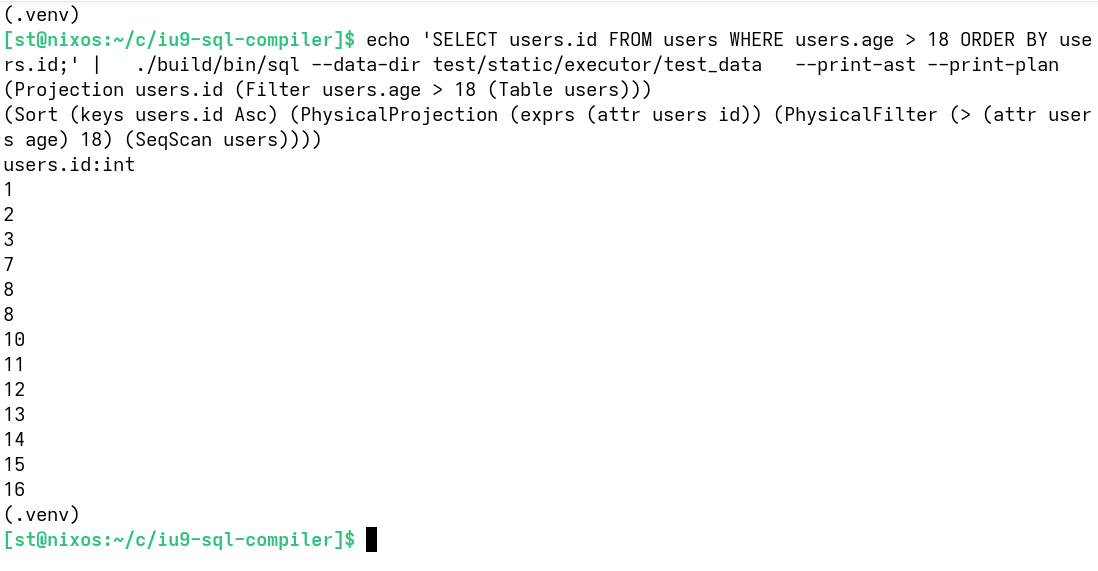
\includegraphics[width=0.8\textwidth]{run-with-prints.png}
% \caption{Вывод логического дерева и физического плана}%
% \label{fig:practice-plan}
% \end{figure}

% Для проверки полноты набора правил оптимизации предусмотрен режим
% \verb|--check-reachable|. В этом режиме программа получает SQL-запрос и
% сериализованный физический план, после чего выполняет полный перебор
% пространства поиска без отсечения по стоимости. Если заданный план может быть
% получен с помощью реализованных правил, программа выводит сообщение
% \verb|REACHABLE|.

% План передается в отдельном файле в формате S-expression. Например, содержимое
% файла \verb|target.plan| может иметь вид, представленный на листинге~\ref{lst:target-plan}.

% \begin{listing}[H]
%   \caption{Пример содержимого файла с целевым физическим планом.}
%   \label{lst:target-plan}
%   \begin{minted}[style=bw, breaklines, frame=single, fontsize=\footnotesize]{text}
% (PhysicalProjection (exprs (attr users id))
%   (PhysicalFilter (> (attr users age) 18)
%     (SeqScan users)))
%   \end{minted}
% \end{listing}

% Проверка выполняется командой на листинге~\ref{lst:check-reachable}.

% \begin{listing}[H]
%   \caption{Запуск программы в режиме проверки достижимости плана.}
%   \label{lst:check-reachable}
%   \begin{minted}[style=bw, breaklines, frame=single, fontsize=\footnotesize]{text}
% echo 'SELECT users.id FROM users WHERE users.age > 18;' | \
%   ./build/bin/sql \
%   --data-dir test/static/executor/test_data \
%   --check-reachable target.plan
%   \end{minted}
% \end{listing}

Если план недостижим, программа выводит сообщение \verb|NOT REACHABLE| и
описание первого обнаруженного расхождения. Параметр \verb|--data-dir|
необходим для загрузки схем таблиц. В частности, схема используется при
проверке достижимости планов с сортировкой.

% Модульные тесты проверяют синтаксический анализ запросов, вычисление выражений,
% исполнение физических операторов, индексное сканирование, сериализацию планов,
% структуру Memo, правила оптимизации и физические свойства.

% Для запуска Python-тестов преобразователя планов Microsoft SQL Server
% необходимо предварительно запустить контейнер, после чего выполнить команды на листинге~\ref{lst:pytest-converter}.

% \begin{listing}[H]
%   \caption{Запуск тестов преобразователя планов Microsoft SQL Server.}
%   \label{lst:pytest-converter}
%   \begin{minted}[style=bw, breaklines, frame=single, fontsize=\footnotesize]{text}
% cd research
% pytest -q test_converter.py
% cd ..
%   \end{minted}
% \end{listing}

% Тесты инструментов Star Schema Benchmark запускаются командой на листинге~\ref{lst:pytest-ssb}.

% \begin{listing}[H]
%   \caption{Запуск тестов инструментов Star Schema Benchmark.}
%   \label{lst:pytest-ssb}
%   \begin{minted}[style=bw, breaklines, frame=single, fontsize=\footnotesize]{text}
% pytest -q benchmarks/datasets/ssb
%   \end{minted}
% \end{listing}

Для поиска ошибок исполнения реализован дифференциальный фаззер. Он генерирует
случайные SQL-запросы, выполняет их в модельной СУБД и Microsoft SQL Server,
после чего сравнивает полученные результаты. Перед запуском необходимо поднять
контейнер с Microsoft SQL Server. Фаззер запускается из корневого каталога
проекта командой на листинге~\ref{lst:reach-fuzz}.

Второй фаззер проверяет полноту набора правил оптимизатора. Он получает
физический план запроса из Microsoft SQL Server, преобразует его во внутренний
формат проекта и запускает программу в режиме \verb|--check-reachable|, как
показано на листинге~\ref{lst:reach-fuzz}.

\begin{listing}[H]
  \caption{Запуск фаззеров.}
  \label{lst:reach-fuzz}
  \begin{minted}[style=bw, breaklines, frame=single, fontsize=\footnotesize]{text}
docker compose up -d
python -m research.fuzz.reach_fuzz \
  --cli build/bin/sql \
  --data-dir test/static/executor/test_data
python -m research.fuzz.diff_fuzz \
  --cli build/bin/sql \
  --data-dir test/static/executor/test_data
  \end{minted}
\end{listing}

% \begin{figure}[H]
% \centering
% 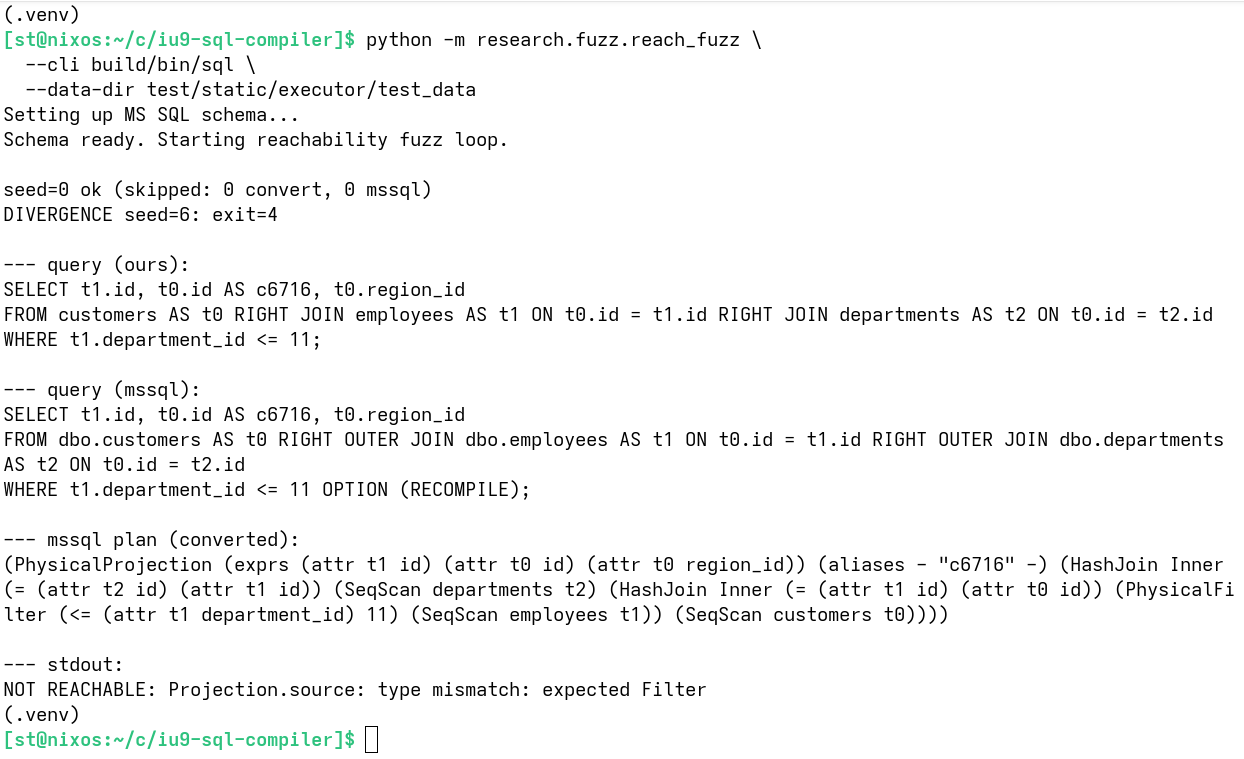
\includegraphics[width=0.8\textwidth]{reach-fuzz.png}
% \caption{Пример вывода фаззера проверки полноты правил оптимизатора}%
% \label{fig:reach-fuzz}
% \end{figure}

% \begin{longtable}{|p{4.2cm}|p{9.3cm}|}
%   \caption{Параметры командной строки программы.}\label{tbl:practice-cli}\\
%   \hline
%   Параметр & Назначение \\
%   \hline
%   \endfirsthead
%   \multicolumn{2}{l}{\small Продолжение таблицы~\ref{tbl:practice-cli}}\\
%   \hline
%   Параметр & Назначение \\
%   \hline
%   \endhead
%   \texttt{--data-dir DIR} &
%   Директория с CSV-файлами таблиц. Обязательна при обычном исполнении запроса. \\
%   \hline
%   \texttt{--print-ast} &
%   Вывод логического дерева операторов после синтаксического анализа. \\
%   \hline
%   \texttt{--print-plan} &
%   Вывод выбранного физического плана в формате S-expression. \\
%   \hline
%   \texttt{--jit} &
%   Использование кэшируемой JIT-компиляции скалярных выражений. \\
%   \hline
%   \texttt{--check-reachable FILE} &
%   Проверка достижимости физического плана, сериализованного в файле. \\
%   \hline
% \end{longtable}

\section{Аналитическая часть}

Тестирование разработанной модельной СУБД выполнялось на нескольких уровнях. Для
проверки отдельных компонентов использовались модульные тесты. Корректность
выполнения запросов и полнота пространства поиска оптимизатора дополнительно
проверялись с помощью фаззинга. Для оценки производительности и калибровки
стоимостной модели были реализованы бенчмарки. Вспомогательные инструменты на
языке Python проверяются с помощью библиотеки \verb|pytest|.

Модульные тесты реализованы с использованием библиотеки GoogleTest. Они
проверяют синтаксический анализ SQL-запросов, исполнение физических операторов,
индексное сканирование, вычисление выражений, сериализацию физических планов,
структуру Memo, правила оптимизации и обработку свойств сортировки. Пример теста
синтаксического анализатора приведен в листинге~\ref{lst:googletest}. Также
проверяется выбор физического плана. Например, при различных оценках
кардинальности оптимизатор должен выбирать подходящий порядок соединения таблиц.

\begin{listing}[H]
  \caption{Пример модульного теста.}
  \label{lst:googletest}
  \begin{minted}[style=bw, breaklines, frame=single, fontsize = \footnotesize, linenos=false, xleftmargin = 1.5em]{cpp}
TEST(ParserTest, SelectSingleColumnFromSingleTable) {
  std::stringstream s{"SELECT users.id FROM users;"};

  Operator got = GetAST(s).value().op;

  ASSERT_THAT(got, VariantWith<Projection>(
      Projection{
          std::vector<Expression>{{Attribute{"users", "id"}}},
          std::make_shared<Operator>(Table{"users"})
      }));
}
  \end{minted}
\end{listing}

Для проверки вспомогательных инструментов используются тесты на языке Python.
Они разделены на две группы. Первая группа проверяет преобразование физических
планов Microsoft SQL Server из формата ShowPlanXML во внутренний текстовый
формат проекта. Рассматриваются последовательное и индексное сканирование,
фильтрация, сортировка, агрегация и соединения. Часть тестов использует заранее
подготовленные XML-фрагменты, часть может быть запущена с подключением к
экземпляру Microsoft SQL Server.

Вторая группа относится к стандартному Star Schema Benchmark. Она проверяет
преобразование исходных таблиц SSB в CSV-формат модельной СУБД, обработку
некорректных входных данных и успешное выполнение стандартных аналитических
запросов.

\subsection{Дифференциальный анализ и тестирование производительности}

Для проверки системы на большом количестве входных данных реализован генератор
случайных SQL-запросов. Он строит запросы из поддерживаемого подмножества языка:
проекции, фильтры, соединения, группировки, агрегатные функции, сортировки,
строковые выражения, \verb|IN| и \verb|BETWEEN|.

% TODO: заменить на макросы \sqkkw

Дифференциальный фаззер выполняет каждый сгенерированный запрос в модельной СУБД
и в Microsoft SQL Server. Результаты сравниваются как мультимножества строк. Для
запросов с \verb|ORDER BY| дополнительно проверяется корректность порядка
результатов.

Отдельный фаззер используется для исследования полноты набора правил
оптимизации. Для случайного запроса из Microsoft SQL Server извлекается
физический план, после чего план преобразуется во внутренний формат проекта.
Затем модельный оптимизатор выполняет полный перебор пространства поиска и
проверяет, достижим ли полученный план с помощью реализованных правил. Такой
подход позволяет находить отсутствующие преобразования и физические операторы.

Тесты производительности реализованы с помощью библиотеки Google Benchmark. Для
запросов предусмотрены два режима построения физического плана: \verb|Naive| и
\verb|Optimized|. В первом случае физический план строится непосредственно по
логическому дереву без применения оптимизатора. Во втором случае используется
стоимостная оптимизация. Сравнение этих режимов позволяет оценить влияние
выбранного физического плана на время выполнения запроса.

Бенчмарки выполняются как для небольших синтетических тестовых запросов, так и
для набора аналитических запросов Star Schema Benchmark. Дополнительно
поддерживается сравнение интерпретируемого и JIT-компилируемого способов
вычисления выражений.

\begin{figure}[H]
\centering
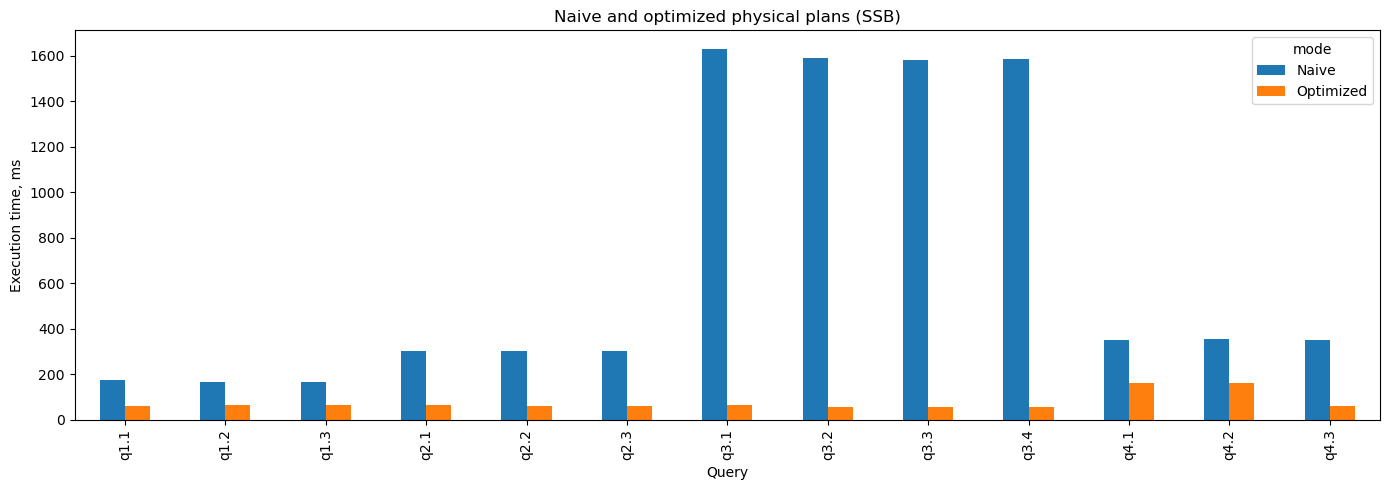
\includegraphics[width=0.8\textwidth]{naive-vs-optimizer.png}
\caption{Сравнение времени выполнения запросов при наивном и оптимизированном
   построении физического плана.}
\label{fig:benchmark-naive-optimized}
\end{figure}

\begin{figure}[H]
\centering
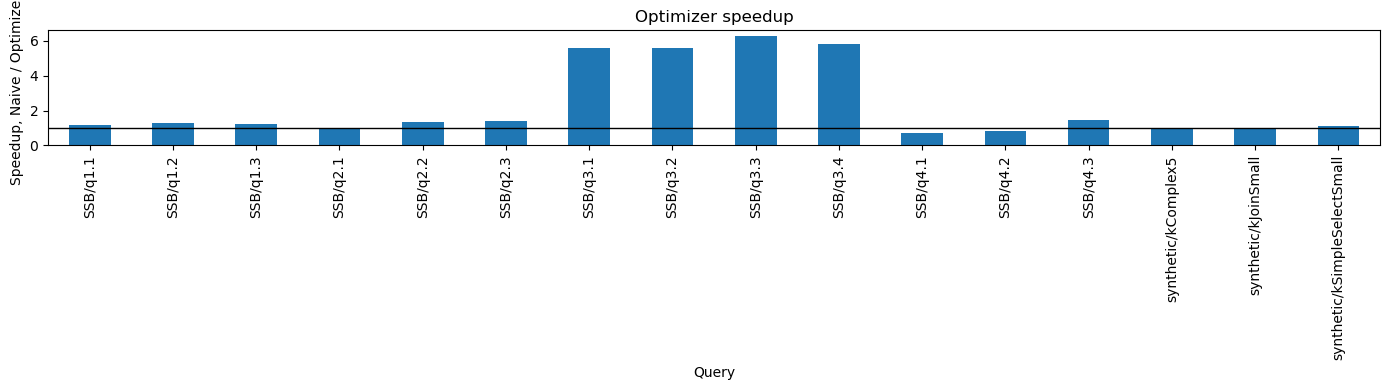
\includegraphics[width=0.8\textwidth]{optimizer-speedup.png}
\caption{Относительное ускорение выполнения запросов после применения оптимизатора.}
\label{fig:benchmark-speedup}
\end{figure}

В таблице~\ref{tbl:ssb-benchmark} приведено среднее время выполнения трех
повторений запросов SSB. Ускорение рассчитывается как отношение времени
выполнения наивного плана ко времени выполнения оптимизированного плана.

Видно, что на стандартном наборе запросов оптимизатор дает улучшение в $1.2-1.5$
раз, а на накоторых запросах в $6$ и более раз.

\begin{table}[H]
  \centering
  \caption{Результаты выполнения запросов Star Schema Benchmark.}
  \label{tbl:ssb-benchmark}
  \begin{tabular}{|l|r|r|r|}
    \hline
    Запрос & \texttt{Naive}, мс & \texttt{Optimized}, мс & Ускорение \\
    \hline
    \texttt{q1.1} & 8.11 & 6.51 & 1.25 \\
    \texttt{q1.2} & 8.20 & 6.59 & 1.24 \\
    \texttt{q1.3} & 8.00 & 6.58 & 1.22 \\
    \texttt{q2.1} & 8.80 & 9.33 & 0.94 \\
    \texttt{q2.2} & 8.84 & 6.18 & 1.43 \\
    \texttt{q2.3} & 8.68 & 5.80 & 1.50 \\
    \texttt{q3.1} & 35.67 & 5.90 & 6.04 \\
    \texttt{q3.2} & 35.88 & 5.58 & 6.43 \\
    \texttt{q3.3} & 38.05 & 5.86 & 6.49 \\
    \texttt{q3.4} & 37.12 & 5.77 & 6.43 \\
    \texttt{q4.1} & 9.06 & 12.21 & 0.74 \\
    \texttt{q4.2} & 9.05 & 11.12 & 0.81 \\
    \texttt{q4.3} & 9.28 & 6.31 & 1.47 \\
    \hline
  \end{tabular}
\end{table}

\subsection{Калибровка стоимостной модели}

Для калибровки коэффициентов в стоимостных формулах реализованы отдельные
бенчмарки физических операторов.
Измеряется время выполнения последовательного сканирования, фильтрации,
проекции, сортировки, агрегации, хеш-соединения, соединения вложенными циклами и
декартова произведения~\refImage{fig:operator-benchmark}.

\begin{figure}[H]
\centering
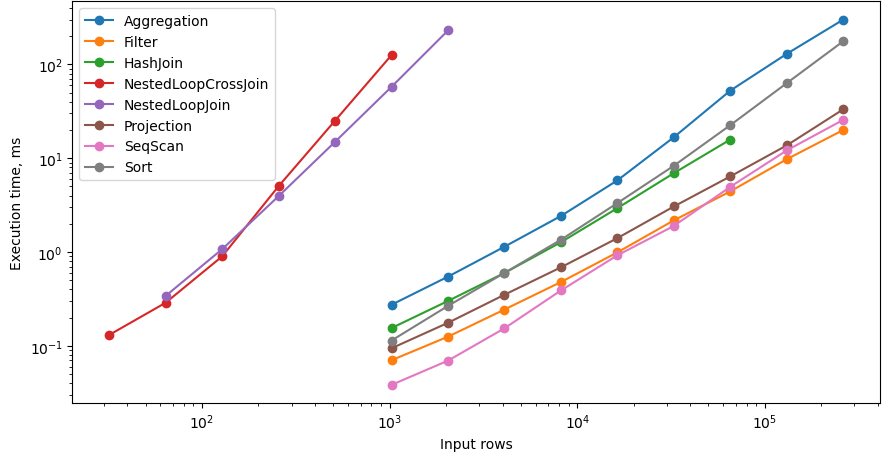
\includegraphics[width=0.7\textwidth]{scaling.png}
\caption{Зависимость времени выполнения физических операторов от размера входных
   данных.}
\label{fig:operator-benchmark}
\end{figure}

При выполнении этих бенчмарков данные хранятся в оперативной памяти. Это
позволяет уменьшить влияние файловой системы и измерять преимущественно
стоимость самого физического оператора. Для каждого оператора выполняются замеры
на таблицах различного размера.

Дополнительно формируются группы запусков с приблизительно одинаковой расчетной
стоимостью. Для этого размер входных отношений выбирается на основе стоимостной
формулы оператора. Сопоставление расчетной стоимости с фактическим временем
выполнения позволяет сравнить операторы между собой и скорректировать
коэффициенты модели~\refImage{fig:cost-model-calibration}. Благодаря этому
оптимизатор принимает решения на основе оценок, соответствующих характеристикам
реализованного исполнителя.

Выведенные коэффициенты дополнительно валидируются на случайных запросах путем
сравнения полной стоимости плана и времени его
исполнения~\refImage{fig:cost-on-random-queries}.

\anonsection{ЗАКЛЮЧЕНИЕ}

В ходе работы была изучена архитектура оптимизаторов Cascades и на ее основе
спроектирован собственный оптимизатор для модельной реляционной СУБД.

Было формализовано поддерживаемое подмножество SQL и соответствующее ему
представление в терминах реляционной алгебры. Реализованная система поддерживает
запросы на чтение данных с основными операторами диалекта PostgreSQL.

Был реализован алгоритм поиска оптимального физического плана и структура Memo
для эффективного хранения групп логически эквивалентных выражений. В результате
система выбирает физический план с минимальной оценочной стоимостью с учетом
требуемых свойств результата.

Для формирования пространства поиска был разработан набор правил трансформации и
реализации для основных операторов реляционной алгебры. Реализованные правила
позволяют изменять порядок и группировку соединений, преобразовывать предикаты и
выражения, а также сопоставлять логическим операторам физические реализации.

Для ускорения поиска был реализован метод ветвей и границ. Оптимизатор
использует текущую лучшую стоимость и нижние оценки стоимости поддеревьев для
отсечения заведомо неоптимальных вариантов, что уменьшает объем исследуемого
пространства планов ухудшения качества результирующих планов.

Для последующего развития оптимизатора был реализован метод дифференциального
анализа физических планов. Подготовлены инструменты генерации запросов,
сравнения результатов исполнения и сопоставления планов с промышленной СУБД
Microsoft SQL Server.

Тем самым цель работы была достигнута. Получена работоспособная и расширяемая
система, которую можно использовать как основу для дальнейшего уточнения правил
оптимизации и увеличения пространства исследуемых планов исполнения запросов.

\renewcommand\refname{СПИСОК ИСПОЛЬЗОВАННЫХ ИСТОЧНИКОВ}
\clearpage
{\catcode`"\active\def"{\relax}
    \addcontentsline{toc}{section}{\protect\numberline{}\refname}%
    \printbibliography
}
\newpage

\settocdepth{section}
\anonsection{ПРИЛОЖЕНИЕ А}
\vspace{-30pt}

\begin{figure}[H]
\centering
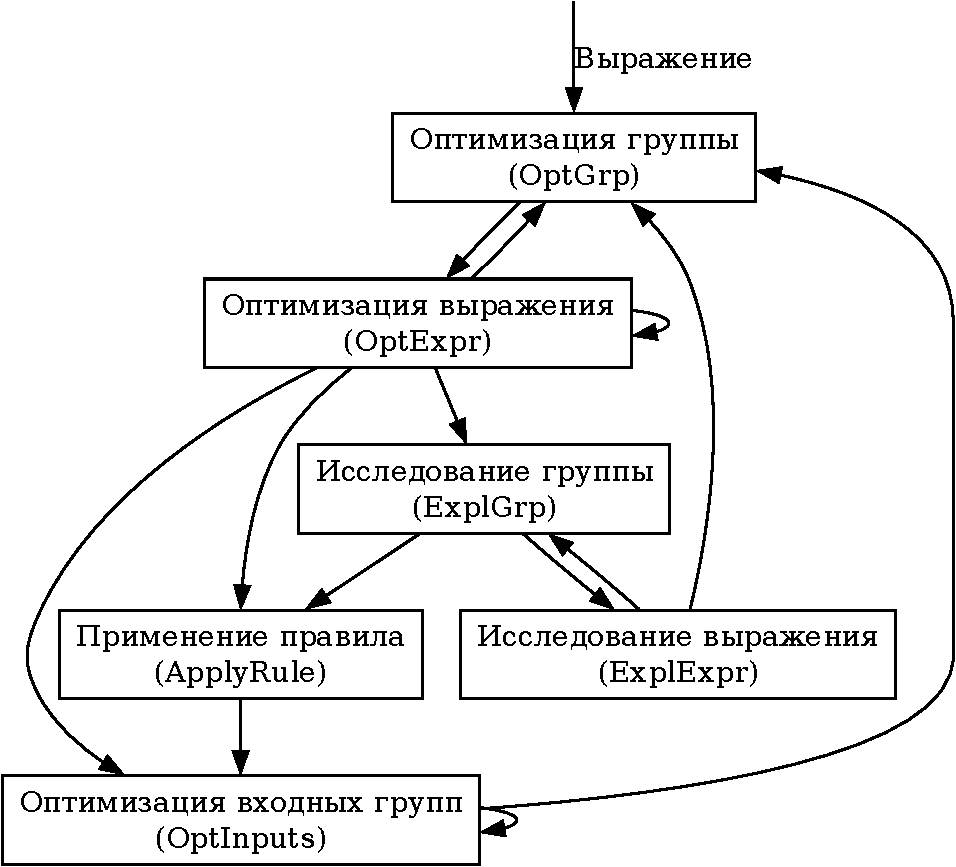
\includegraphics[width=0.7\textwidth]{cascades.pdf}
\caption{Схема взаимодействия задач в оптимизаторе Cascades}%
\label{fig:cascades-tasks}
\end{figure}

\begin{figure}[H]
    \centering
    \begin{tikzpicture}[
        scale=0.85, transform shape,
        group/.style={draw, rounded corners, text width=4.8cm, inner sep=5pt},
        arrow/.style={-{Stealth[length=2.5mm]}, thick},
        altarrow/.style={-{Stealth[length=2.5mm]}, thick, dashed}
    ]
        \node[group] (g5) at (6,0) {
            \textbf{Группа G5}\\[2pt]
            \hrule\vspace{2pt}
            \textit{Логические:}\\
            Join(G4,G3)\\
            Join(G1,G6)\\[2pt]
            \hrule\vspace{2pt}
            \textit{Физические:}\\
            HashJoin(G4,G3)\\
            NestedLoopJoin(G4,G3)\\
            HashJoin(G1,G6)\\
            NestedLoopJoin(G1,G6)
        };
        \node[group] (g4) at (3,-5.4) {
            \textbf{Группа G4}\\[2pt]
            \hrule\vspace{2pt}
            \textit{Логические:}\\
            Join(G1,G2)\\[2pt]
            \hrule\vspace{2pt}
            \textit{Физические:}\\
            HashJoin(G1,G2)\\
            NestedLoopJoin(G1,G2)
        };
        \node[group] (g6) at (9,-5.4) {
            \textbf{Группа G6}\\[2pt]
            \hrule\vspace{2pt}
            \textit{Логические:}\\
            Join(G2,G3)\\[2pt]
            \hrule\vspace{2pt}
            \textit{Физические:}\\
            HashJoin(G2,G3)\\
            NestedLoopJoin(G2,G3)
        };
        \node[group] (g1) at (0,-9.8) {
            \textbf{Группа G1}\\[2pt]
            \hrule\vspace{2pt}
            \textit{Логические:}\\
            Scan(A)\\[2pt]
            \hrule\vspace{2pt}
            \textit{Физические:}\\
            SeqScan(A)
        };
        \node[group] (g2) at (6,-9.8) {
            \textbf{Группа G2}\\[2pt]
            \hrule\vspace{2pt}
            \textit{Логические:}\\
            Scan(B)\\[2pt]
            \hrule\vspace{2pt}
            \textit{Физические:}\\
            SeqScan(B)
        };
        \node[group] (g3) at (12,-9.8) {
            \textbf{Группа G3}\\[2pt]
            \hrule\vspace{2pt}
            \textit{Логические:}\\
            Scan(C)\\[2pt]
            \hrule\vspace{2pt}
            \textit{Физические:}\\
            SeqScan(C)
        };

        \draw[arrow] (g5) -- (g4);
        \draw[arrow, rounded corners=5pt]
            (g5.east) -- (15.5,0) -- (15.5,-9.8) -- (g3.east);
        \draw[altarrow] (g5) -- (g6);
        \draw[altarrow, rounded corners=5pt]
            (g5.west) -- (-3.5,0) -- (-3.5,-9.8) -- (g1.west);
        \draw[arrow] (g4) -- (g1);
        \draw[arrow] (g4) -- (g2);
        \draw[arrow] (g6) -- (g2);
        \draw[arrow] (g6) -- (g3);
    \end{tikzpicture}
    \caption{Пример структуры Memo.}%
    \label{fig:memo-structure}
\end{figure}

\begin{table}[H]
  \centering
  \caption{Формулы оценки селективности предикатов.}
  \label{tbl:selectivity-model}
  \small
  \begin{tabular}{|p{0.42\textwidth}|p{0.42\textwidth}|}
    \hline
    Вид предиката & Формула селективности \\
    \hline
    \(a = c\), где \(a\) --- атрибут, \(c\) --- константа
      & \(sel(a = c) = 0{,}10\) \\
    \hline
    \(a < b\), \(a > b\), \(a \le b\), \(a \ge b\)
      & \(sel(p) = 0{,}50\) \\
    \hline
    \(p_1 \land p_2\)
      & \(sel(p_1 \land p_2) = sel(p_1) \cdot sel(p_2)\) \\
    \hline
    \(p_1 \lor p_2\)
      & \(sel(p_1 \lor p_2) =
         sel(p_1) + sel(p_2) - sel(p_1) \cdot sel(p_2)\) \\
    \hline
    \(\lnot p\)
      & \(sel(\lnot p) = 1 - sel(p)\) \\
    \hline
    \(a \in \{c_1, \ldots, c_k\}\)
      & \(sel(p) = \min(0{,}50,\; 0{,}10k)\) \\
    \hline
    \(a \notin \{c_1, \ldots, c_k\}\)
      & \(sel(p) = 1 - \min(0{,}50,\; 0{,}10k)\) \\
    \hline
    \(a = b\) в условии соединения, где \(a\) и \(b\) --- атрибуты разных входов
      & \(sel(a = b) = \frac{1}{\max(1,\; \max(n_l, n_r))}\) \\
    \hline
    \(\theta_1 \land \theta_2\) в условии соединения
      & \(sel(\theta_1 \land \theta_2) =
         sel(\theta_1) \cdot sel(\theta_2)\) \\
    \hline
    Иной или неизвестный предикат фильтрации
      & \(sel(p) = 0{,}50\) \\
    \hline
    Иной или неизвестный предикат соединения
      & \(sel(\theta) = 1\) \\
    \hline
  \end{tabular}
\end{table}


\begin{algorithm}[H]
    \caption{Алгоритм поиска (часть 1).}%
    \label{alg:cascades-search}
    \begin{algorithmic}[1]
    \Procedure{Optimize}{$root, required$}
        \State Push task $\Call{OptimizeGroup}{root.group, required, +\infty}$
        \While{task stack is not empty}
            \State Pop and execute top task
        \EndWhile
        \State \Return $\Call{BuildPlan}{root.group, required}$
    \EndProcedure

    \Procedure{ExploreGroup}{$group, limit$}
        \State Mark $group$ as explored
        \For{each logical expression $expr \in group$}
            \State Push task $\Call{ExploreExpression}{expr, limit}$
        \EndFor
    \EndProcedure

    \Procedure{ExploreExpression}{$expr, limit$}
        \State $\Call{TryRules}{expr, limit}$
        \If{$expr$ is already explored}
            \State \Return
        \EndIf
        \State Mark $expr$ as explored
        \For{each $child \in \Call{Children}{expr}$}
            \State Register $expr$ as parent of $child$
            \If{$child$ is not explored}
                \State Push task $\Call{ExploreGroup}{child, limit}$
            \EndIf
        \EndFor
    \EndProcedure

    \Procedure{TryRules}{$expr, limit$}
        \For{each applicable transformation rule $r$}
            \State Push task $\Call{ApplyTransformation}{r, expr, limit}$
        \EndFor
        \For{each applicable implementation rule $r$}
            \State Push task $\Call{ApplyImplementation}{r, expr}$
        \EndFor
    \EndProcedure
    \end{algorithmic}
\end{algorithm}

\begin{algorithm}[H]
    \caption{Алгоритм поиска (часть 2).}%
    \label{alg:cascades-search-2}
    \begin{algorithmic}[1]
    \Procedure{OptimizeGroup}{$group, required, limit$}
        \If{$winner[group, required]$ exists \textbf{or} $group$ is explored \textbf{and} $\Call{LowerBound}{group} \geq limit$}
            \State \Return
        \EndIf
        \If{$group$ is not explored}
            \State Push task $\Call{OptimizeGroup}{group, required, limit}$
            \State Push task $\Call{ExploreGroup}{group, limit}$
            \State \Return
        \EndIf
        \For{each physical expression $phys \in group$}
            \If{$phys$ is not enforcer \textbf{and} $local\_cost[phys] < limit$}
                \State Push task $\Call{OptimizeInputs}{phys, required, \varnothing, local\_cost[phys], limit, 0}$
            \EndIf
        \EndFor
        \For{each enforcer applicable to $(group, required)$}
            \State Add enforcer expression $phys$ and compute $local\_cost[phys]$
            \If{$local\_cost[phys] < limit$}
                \State Push task $\Call{OptimizeInputs}{phys, required, \varnothing, local\_cost[phys], limit, 0}$
            \EndIf
        \EndFor
    \Procedure{OptimizeInputs}{$phys, required, delivered, accum, limit, i$}
        \If{$winner[phys.group, required]$ exists}
            \State $limit \leftarrow \min(limit,\; winner[phys.group, required].cost)$
        \EndIf
        \If{$accum \geq limit$}
            \State \Return
        \EndIf
        \If{$i = |children|$}
            \State $props \leftarrow \Call{DeriveOutputProps}{phys, delivered}$
            \State Update winner and \Return
        \EndIf
        \State Calc child limit and requirements
        \State Push task $\Call{OptimizeGroup}{child, child\_required, child\_limit}$
    \EndProcedure
    \EndProcedure

    \end{algorithmic}
\end{algorithm}

\begin{scriptsize}
\begin{longtable}{|c|p{2.6cm}|c|p{4.2cm}|}
  \caption{Правила трансформации.}\label{tbl:transformation_rules}\\
  \hline
  № & Название & Правило & Комментарий \\
  \hline
  \endfirsthead
  \multicolumn{4}{l}{\small Продолжение таблицы~\ref{tbl:transformation_rules}}\\
  \hline
  № & Название & Правило & Комментарий \\
  \hline
  \endhead
  \hline
  \endfoot
  \hline
  \endlastfoot

  1 & Коммутативность соединения &
    \(\TransRule{\InnerJoin{R}{\theta}{S}}{\text{внутреннее или полное внешнее соединение}}{\InnerJoin{S}{\theta}{R}}\) &
    Перестановка входов соединения. Позволяет рассмотреть оба порядка вычисления. \\
  \hline

  2 & Ассоциативность соединения &
    \(\TransRule{\InnerJoin{(\InnerJoin{R}{\theta_1}{S})}{\theta_2}{T}}{\substack{\text{оба соединения внутренние;}\\ \theta_1 \land \theta_2 \text{ перераспределяемы}}}{\InnerJoin{R}{\theta'_1}{(\InnerJoin{S}{\theta'_2}{T})}}\) &
    Изменяет группировку цепочки соединений. Открывает альтернативные порядки и уменьшает размер промежуточных результатов. \\
  \hline

  3 & Проталкивание фильтра в левый вход &
    \(\TransRule{\Sel{p}{\InnerJoin{R}{\theta}{S}}}{\substack{attrs(p) \subseteq attrs(R); \\ \text{внутреннее соединение или сохраняющий вход}}}{\InnerJoin{\Sel{p}{R}}{\theta}{S}}\) &
    Применяет селективный предикат до соединения, уменьшая кардинальность входа. \\
  \hline

  4 & Проталкивание фильтра в правый вход &
    \(\TransRule{\Sel{p}{\InnerJoin{R}{\theta}{S}}}{\substack{attrs(p) \subseteq attrs(S); \\ \text{внутреннее соединение или сохраняющий вход}}}{\InnerJoin{R}{\theta}{\Sel{p}{S}}}\) &
    Симметричный случай для правого входа. \\
  \hline

  5 & Перенос фильтра в предикат соединения &
    \(\TransRule{\Sel{p}{\InnerJoin{R}{\theta}{S}}}{\substack{\text{соединение внутреннее;} \\ attrs(p) \subseteq attrs(R) \cup attrs(S)}}{\InnerJoin{R}{\theta \land p}{S}}\) &
    Объединяет фильтр и предикат соединения. Может позволить применить хеш-соединение или соединение слиянием. \\
  \hline

  6 & Превращение декартова произведения в соединение &
    \(\TransRule{\Sel{p}{\CProd{R}{S}}}{\top}{\InnerJoin{R}{p}{S}}\) &
    Частный случай правила~5. \\
  \hline

  7 & Поднятие фильтра над соединением &
    \(\TransRule{\InnerJoin{\Sel{p}{R}}{\theta}{S}}{\substack{attrs(p) \subseteq attrs(R); \\ \text{внутреннее соединение или сохраняющая сторона}}}{\Sel{p}{\InnerJoin{R}{\theta}{S}}}\) &
    Переносит фильтр выше соединения для объединения с предикатами родительских операторов. \\
  \hline

  8 & Разбиение фильтра на конъюнкты &
    \(\TransRule{\Sel{p_1 \land \ldots \land p_n}{R}}{\top}{\Sel{p_1}{\ldots \Sel{p_n}{R} \ldots}}\) &
    Позволяет обрабатывать каждый конъюнкт независимо. \\
  \hline

  9 & Проталкивание проекции через соединение &
    \(\TransRule{\Projection{L}{\InnerJoin{R}{\theta}{S}}}{\substack{L_R \cup J_R \subsetneq attrs(R) \\ \text{или}\ L_S \cup J_S \subsetneq attrs(S)}}{\Projection{L}{\InnerJoin{\Projection{L_R \cup J_R}{R}}{\theta}{\Projection{L_S \cup J_S}{S}}}}\) &
    Удаляет неиспользуемые атрибуты до соединения, сокращая ширину кортежей. \\
  \hline

  10 & Левое внешнее соединение во внутреннее &
    \(\TransRule{\Sel{p}{\LOJ{R}{\theta}{S}}}{p\ \text{null-отбрасывающий по}\ attrs(S)}{\Sel{p}{\InnerJoin{R}{\theta}{S}}}\) &
    Открывает для подплана правила, ограниченные внутренним соединением. \\
  \hline

  % 11 & Правое внешнее соединение во внутреннее &
  %   \(\TransRule{\Sel{p}{\ROJ{R}{\theta}{S}}}{p\ \text{null-отбрасывающий по}\ attrs(R)}{\Sel{p}{\InnerJoin{R}{\theta}{S}}}\) &
  %   Симметричный случай. \\
  % \hline

  11 & Полное внешнее соединение во внутреннее &
    \(\TransRule{\Sel{p}{\FOJ{R}{\theta}{S}}}{p\ \text{null-отбрасывающий по}\ attrs(R)\ \text{и}\ attrs(S)}{\Sel{p}{\InnerJoin{R}{\theta}{S}}}\) &
    Требует null-отбрасывания с обеих сторон. \\
  \hline

  12 & Проталкивание агрегации ниже соединения &
    \(\TransRule{\Agg{G}{F}{\InnerJoin{R}{R.k = S.k}{S}}}{\substack{F\text{ разделяема;}\\ \text{внутреннее соединение по равенству}}}{\Agg{G}{F'}{\InnerJoin{\AggP{G_R \cup \{R.k\}}{F_R}{R}}{R.k=S.k}{S}}}\) &
    Снижает кардинальность входа частичной группировкой. \(G_R = G \cap attrs(R)\); \(F_R\) --- частичные агрегаты по атрибутам \(R\); \(F'\) --- финальные комбинаторы. \\
  \hline

  13 & Перестановка агрегации и соединения &
    \(\TransRule{\Agg{G}{F_R}{\InnerJoin{R}{R.k=S.k}{S}}}{\substack{\text{внутреннее соединение по равенству;}\\ F_R\subseteq attrs(R);\ R.k \in G; \\ S.k\text{ уникален и полон}}}{\InnerJoin{\Agg{G}{F_R}{R}}{R.k=S.k}{S}}\) &
    Полностью переносит агрегацию до соединения. \(S.k\) уникален: соединение не дублирует строки \(R\). \(S.k\) полон относительно \(R.k\): соединение не теряет строки \(R\). \\
  \hline
\end{longtable}

\begin{table}[H]
  \centering
  \caption{Стоимостные формулы физических операторов.}
  \label{tbl:cost-model-coefficients}
  \small
  \begin{tabular}{|p{0.40\textwidth}|l|}
    \hline
    Физический оператор & Формула стоимости \\
    \hline
    Последовательное сканирование & $100\,n$ \\
    Фильтрация                    & $100\,n_{out}$ \\
    Проекция                      & $22\,n_{out}$ \\
    Сортировка                    & $11\,n\bigl(\lfloor\log_2 n\rfloor + 1\bigr)$ \\
    Агрегация                     & $510\,n$ \\
    Потоковая агрегация           & $130\,n$ \\
    Соединение вложенными циклами & $70\,n_l n_r$ \\
    Соединение слиянием           & $18\,n_l + n_l\,+ 10\,n_o w_o$ \\
    Декартово произведение        & $104\,n_l n_r$ \\
    Хеш-соединение                & $100\,n_b w_b + 35\,n_p + 10\,n_o w_o$ \\
    \hline
  \end{tabular}
\end{table}

\begin{longtable}{|c|p{2.8cm}|c|p{4.5cm}|}
  \caption{Правила реализации.}\label{tbl:implementation_rules}\\
  \hline
  № & Название & Правило & Комментарий \\
  \hline
  \endfirsthead
  \multicolumn{4}{l}{\small Продолжение таблицы~\ref{tbl:implementation_rules}}\\
  \hline
  № & Название & Правило & Комментарий \\
  \hline
  \endhead
  \hline
  \endfoot
  \hline
  \endlastfoot

  1 & Последовательное сканирование &
    \(\TransRule{\LogicalGet}{\top}{\SeqScan}\) &
    Применимо к любому отношению. \\
  \hline

  2 & Сканирование по индексу &
    \(\TransRule{\LogicalGet}{\text{есть совместимый индекс}}{\IndexScan}\) &
    Индекс должен быть совместим с предикатом или требуемым порядком. \\
  \hline

  3 & Соединение вложенными циклами &
    \(\TransRule{\InnerJoin{R}{\theta}{S}}{\top}{\NestedLoopJoin}\) &
    Применимо при любом виде предиката. Стоимость высока без доступа по индексу к внутреннему отношению. \\
  \hline

  4 & Хеш-соединение &
    \(\TransRule{\InnerJoin{R}{\theta}{S}}{\theta\ \text{содержит равенство по ключам}}{\HashJoin}\) &
    Хеш-таблица строится по ключам равенства. \\
  \hline

  5 & Соединение слиянием &
    \(\TransRule{\InnerJoin{R}{\theta}{S}}{\text{входы упорядочены по ключам соединения}}{\MergeJoin}\) &
    Требуемый порядок может быть обеспечен явным оператором \Sort{}. \\
  \hline

  6 & Хеш-агрегация &
    \(\TransRule{\Agg{G}{F}{R}}{\top}{\sqlkw{HashAggregate}}\) &
    Не требует упорядоченности входа. Потребляет память пропорционально числу групп. \\
  \hline

  7 & Потоковая агрегация &
    \(\TransRule{\Agg{G}{F}{R}}{\text{вход упорядочен по } G}{\sqlkw{StreamAggregate}}\) &
    Эффективна при уже отсортированном входе. Может быть выгодна, если требуемый порядок нужен и родительскому оператору. \\
  \hline
\end{longtable}
\end{scriptsize}

\begin{listing}[H]
  \caption{Вычисление локальной стоимости физических операторов.}
  \label{lst:optimizer-cost}
  \begin{minted}[style=bw, breaklines, frame=single,
    fontsize=\footnotesize, linenos=false, xleftmargin=1.5em]{cpp}
int64_t CalcCost(PhysicalExpr* expr, CardinalityEstimates& cardinality) {
  return std::visit(utils::Overloaded{
    [&](const physical::NestedLoopJoin& j) {
      return 70 * cardinality.GetCardinality(j.lhs)
                * cardinality.GetCardinality(j.rhs);},
    [&](const physical::HashJoin& j) {
      return 69 * (cardinality.GetCardinality(j.lhs)
                  + cardinality.GetCardinality(j.rhs));}, ...
  \end{minted}
\end{listing}

\begin{figure}[H]
\centering
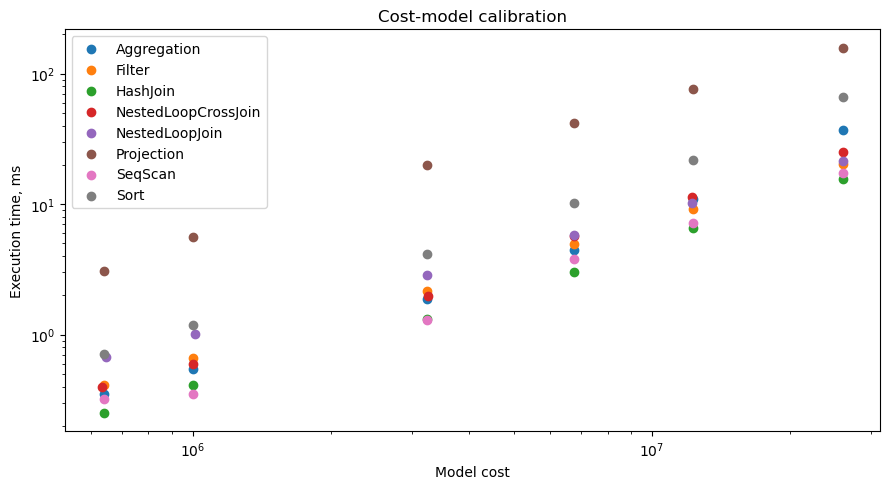
\includegraphics[width=0.8\textwidth]{calibration.png}
\caption{Сопоставление расчетной стоимости физических операторов с фактическим
   временем выполнения.}
\label{fig:cost-model-calibration}
\end{figure}

\begin{listing}[H]
  \caption{Правило коммутативности соединения.}
  \label{lst:join-commutativity}
  \begin{minted}[style=bw, breaklines, frame=single, fontsize=\footnotesize,
    linenos=false, xleftmargin=1.5em]{cpp}
LogicalOperator JoinCommutativity::ApplyImpl(utils::NotNull<LogicalExpr*> expr, Memo&) {
  auto join = std::get<logical::Join>(expr->root_operator);
  std::swap(join.lhs, join.rhs);
  if (join.type == JoinType::kLeft) {
    join.type = JoinType::kRight;
  } else if (join.type == JoinType::kRight) {
    join.type = JoinType::kLeft;
  }
  return join;
}
bool ImplementHashJoin::IsApplicable(utils::NotNull<LogicalExpr*> expr) {
  if (!std::holds_alternative<logical::Join>(expr->root_operator))
    return false;
  const auto& join = std::get<logical::Join>(expr->root_operator);
  if (join.type != JoinType::kInner) return false;
  const auto* bin = std::get_if<BinaryExpression>(&join.qual);
  return bin && bin->binop == BinaryOp::kEq && std::holds_alternative<Attribute>(*bin->lhs) && std::holds_alternative<Attribute>(*bin->rhs);
}
  \end{minted}
\end{listing}

\begin{figure}[H]
\centering
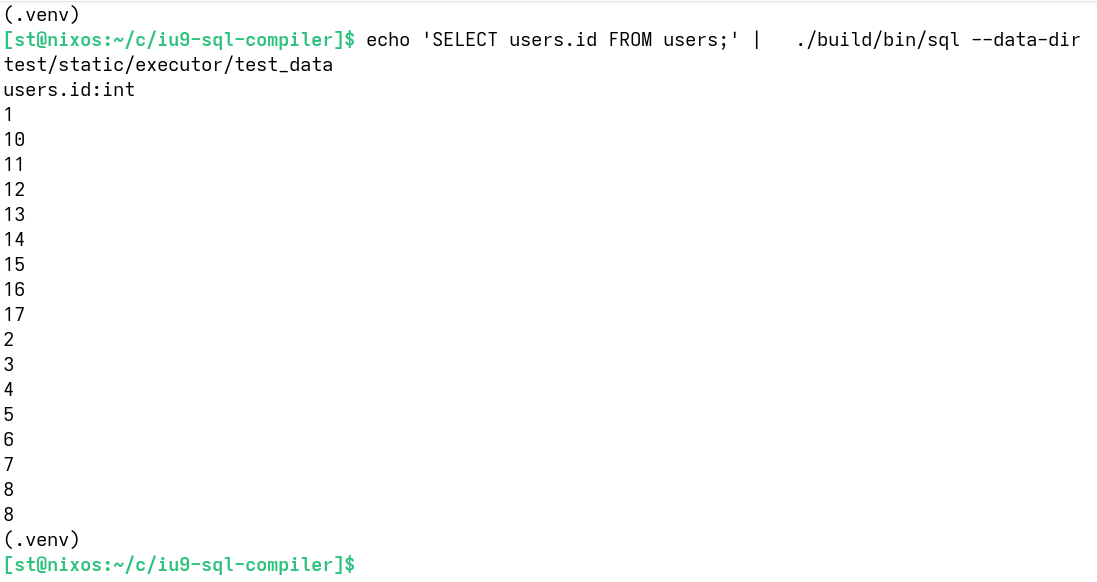
\includegraphics[width=0.8\textwidth]{run-example.png}
\caption{Выполнение SQL-запроса над тестовыми данными}%
\label{fig:practice-run}
\end{figure}

\begin{listing}[H]
  \caption{Оптимизация группы Memo.}
  \label{lst:optimize-group}
  \begin{minted}[style=bw, breaklines, frame=single,
    fontsize=\footnotesize, linenos=false, xleftmargin=1.5em]{cpp}
void Optimizer::OptimizeGroup(Group* group, PropertySet required,
                              Limit limit) {
  WinnerKey key{group, required};
  if (winner_.contains(key)) return;
  if (IsExplored(group) && limit && LowerBoundCost(group) >= *limit) return;
  if (!IsExplored(group)) {
    tasks_.emplace([=] {
      OptimizeGroup(group, required, limit);
    });
    tasks_.emplace([=] {
      ExploreGroup(group, limit);
    });
    return;
  }
  for (auto expr : group->GetPhysicalExprs()) {
    if (expr->is_enforcer) continue;
    auto cost = local_cost_[expr.get()];
    if (!limit || cost < *limit) {
      tasks_.emplace([=] {
        OptimizeInputs(expr, required, {}, cost, limit);
      });
    }
  }
  AddEnforcers(group, required, limit);
}
  \end{minted}
\end{listing}

\begin{figure}[H]
\centering
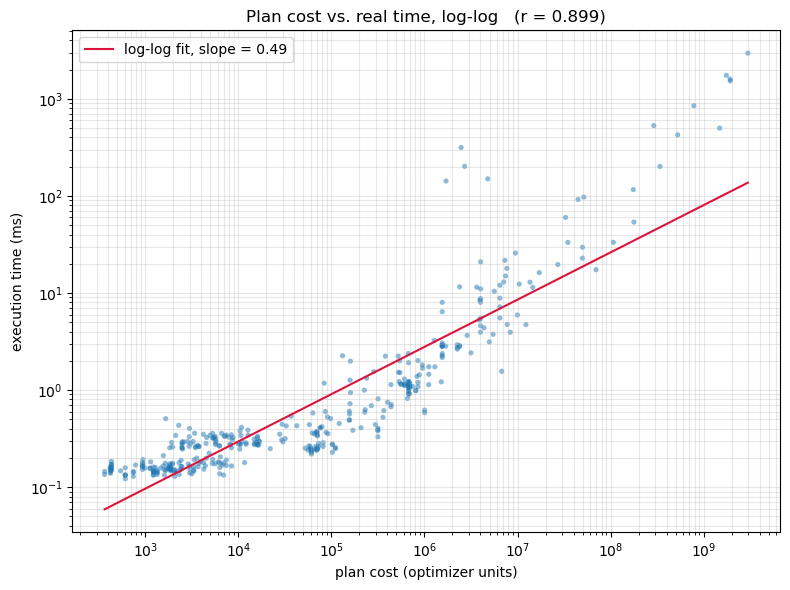
\includegraphics[width=0.7\textwidth]{cost-on-random-queries.png}
\caption{Сравнение скорости выполнения и стоимости на случайных запросах.}%
\label{fig:cost-on-random-queries}
\end{figure}


\end{document}
